\NeedsTeXFormat{LaTeX2e}
%-----------------------------------------------------------
\documentclass[a4paper,12pt]{monografia}
\usepackage[portuguese, colorinlistoftodos, textsize=tiny]{todonotes}
\usepackage{amsmath,amsthm,amsfonts,amssymb}
\usepackage[mathcal]{eucal}
\usepackage{latexsym}
\usepackage[portuguese]{babel}
\usepackage[utf8]{inputenc}
\usepackage{setspace}
%\usepackage{natbib}
\usepackage{bm}
\usepackage[portuguese,algoruled,longend, linesnumbered]{algorithm2e}
\usepackage{listings}
\usepackage{graphicx}
\usepackage{hyperref}
\hypersetup{colorlinks,
  debug=false,
  linkcolor=black,  %%% cor do tableofcontents, \ref, \footnote, etc
  citecolor=black,  %%% cor do \cite
  urlcolor=black,   %%% cor do \url e \href
  bookmarksopen=true,
}
\usepackage[alf,bibjustif]{abntex2cite}

\newcounter{todocounter}
\newcommand{\comment}[2][]
{\stepcounter{todocounter}\todo[caption={\thetodocounter: #2}, #1]
  {
    \begin{spacing}{1}\thetodocounter: #2
\end{spacing}}}
\reversemarginpar
\setlength{\marginparwidth}{2.5cm}
\lstloadlanguages{C}
%-----------------------------------------------------------
%-----------------------------------------------------------
\theoremstyle{plain}
\newtheorem{theorem}{Teorema}[section]
\newtheorem{axiom}{Axioma}[section]
\newtheorem{corollary}{Corolário}[section]
\newtheorem{lemma}{Lema}[section]
\newtheorem{proposition}{Proposição}[section]
%-----------------------------------------------------------
\theoremstyle{definition}
\newtheorem{definition}{Definição}[section]
\newtheorem{example}{Exemplo}[section]
%-----------------------------------------------------------
\theoremstyle{remark}
\newtheorem{remark}{Observação}[section]
%-----------------------------------------------------------
%-----------------------------------------------------------
\newcommand{\R}{\mathbb{R}}
\newcommand{\N}{\mathbb{N}}
\newcommand{\Z}{\mathbb{Z}}
\newcommand{\Q}{\mathbb{Q}}
\newcommand{\K}{\mathbb{K}}
\newcommand{\I}{\mathbb{I}}
\newcommand{\id}{\mathbf{1}}
\newcommand{\U}{\mathcal{U}}
\newcommand{\V}{{\cal V}}
%-----------------------------------------------------------
\def\ind{\hbox{ ind }}
%-----------------------------------------------------------
\hyphenation{Con-si-de-ra-mos}
\hyphenation{me-lhor}
\hyphenation{res-pos-ta}
\hyphenation{re-qui-si-tos}


\begin{document}
%%%%%%%%%%%%%%%%%%%%%%%%%%%%%%%%%%%%%%%%%%%%%%%%%%%%%%%%%%%5
%
%                  INFORMAÇÕES PRÉ-TEXTUAIS
%
%----------------- Título e Dados do Autor -----------------
\titulo{Inteligência artificial aplicada à detecção e classificação de animais em ambiente confinado}

\autor{Vinícius Latini Gonçalves} \nome{Vinícius} \ultimonome{Gonçalves}
%
%---------- Informe o Curso e Grau -----
\bacharelado
\curso{Ciência da Computação} 
\dia{15} \mes{Outubro} \ano{2026} % data da aprovação
\cidade{Juiz de Fora}
%
%----------Informações sobre a Instituição -----------------
\instituicao{Universidade Federal de Juiz de Fora} \sigla{UFJF}
\unidadeacademica{Instituto de Ciências Exatas}
\departamento{Departamento de Ciência da Computação}

%
%------Nomes do Orientador, 1o. Examinador e 2o. Examinador-
\orientador{Luciana Conceição Dias Campos}
\ttorientador{$<<$Título do Orientador$>>$}
%
\coorientador{Érica da Costa Reis Carvalho} % opcional
\ttcoorientador{Doutora em Modelagem Computacional} % se digitado \coorientador
%
\examinadorum{$<<$Nome do Examinador 1$>>$}
\ttexaminadorum{$<<$Título do Examinador 1$>>$}
%
\examinadordois{$<<$Nome do Examinador 2$>>$}
\ttexaminadordois{$<<$Título do Examinador 2$>>$}
%
\examinadortres{Nome do Examinador 3}
\ttexaminadortres{Título do Examinador 3}
%
\examinadorquatro{Nome do Examinador 4}
\ttexaminadorquatro{Título do Examinador 4}
%
%-------- Informações obtidas na Biblioteca ----------------
%
%\CDU{536.21} \areas{1.Análise Matemática  2. Topologia.}
%\npaginas{xx}  % total de páginas do trabalho
%
%%%%%%%%%%%%%%%%%%%%%%%%%%%%%%%%%%%%%%%%%%%%%%%%%%%%%%%%
%    DADOS DE FORMATACAO DA MONOGRAFIA
%
% A instrução abaixo insere a logo do curso e da instituicao na capa da monografia. Basta comentar caso não queira os logos. Para alterar o logo da instituicao e curso, basta alterar os arquivos logoInstituicao.png e logoCurso.jpg. Caso deseje alterar os arquivos, os substituta por imagens do mesmo tamanho!
%\inserirlogo  
%
%
%
%          FIM DAS INFORMAÇÕES PRÉ-TEXTUAIS
%
%%%%%%%%%%%%%%%%%%%%%%%%%%%%%%%%%%%%%%%%%%%%%%%%%%%%%%%%%

\maketitle







%----------------------------dedicatória  opcional--------------
\begin{dedicatoria}
  Aos meus amigos e irmãos.\\
  Aos pais, pelo apoio e sustento.\\
\end{dedicatoria}

%--------Digite aqui o seu resumo em Português--------------
\resumo{Resumo}
O presente trabalho propõe o desenvolvimento de um sistema de baixo custo baseado em Visão Computacional e Inteligência Artificial para detecção e classificação de cabras da raça \textit{Saanen} em confinamento. A iniciativa proposta integra conhecimentos das áreas de Ciência da Computação e Zootecnia, utilizando vídeos capturados em ambientes experimentais para a construção de um banco de imagens rotuladas. Modelos de aprendizado de máquina serão treinados para identificar os caprinos e comparar essas predições com os resultados anotados previamente. Dessa forma, espera-se construir uma ferramenta que possa auxiliar tanto na detecção quanto na classificação desses animais.

\noindent \\ \textbf{Palavras-chave:} Visão Computacional, Inteligência Artificial, Aprendizado de Máquina, Detecção de Objetos, Caprinos \textit{Saanen}, Pecuária de Precisão.

%-----------Digite aqui o seu resumo em Inglês--------------
\resumo{Abstract} This work proposes the development of a low-cost system based on Computer Vision and Artificial Intelligence for the detection and classification of \textit{Saanen} goats in confinement. The proposed initiative combines knowledge from Computer Science and Animal Science, using videos captured in experimental environments to build a labeled image dataset. Machine learning models will be trained to identify the goats, and their predictions will be compared with previously annotated results. In this way, the goal is to build a tool that can support both the detection and the classification of these animals.

\noindent \\ \textbf{Keywords:} Computer Vision, Artificial Intelligence, Machine Learning, Object Detection, \textit{Saanen} Goats, Precision Livestock Farming.

%-----------Ou digite aqui o seu resumo em Frances----------
%\resumo{Resumo} C'est un modúle de la monographie dans \LaTeX et
%5utilise la classe monografia.cls, avec le but de aider dans le
%maniement des travaux de conclusion des plusieurs cours de
%l'Université Fédérale de Juiz de Fora.

%-----------------------------------------------------------
\agradecimento{Agradecimentos} \indent\indent
A todos os meus parentes, pelo encorajamento e
apoio.

Ao professor Beltrano pela orientação, amizade e
principalmente, pela paciência, sem a qual este trabalho não se
realizaria.

Aos professores do Departamento de Ciência da Computação pelos seus
ensinamentos e aos funcionários do curso, que durante esses anos,
contribuíram de algum modo para o nosso enriquecimento pessoal e
profissional.
\newpage

%---------------------- EPÍGRAFE I (OPCIONAL)--------------
\begin{epigrafe}
  ``Lembra que o sono é sagrado e alimenta de horizontes o tempo acordado de viver''.\\
  \hfill Beto Guedes (Amor de Índio)
\end{epigrafe}

%----Sumário, lista de figura e de tabela ------------
\tableofcontents \thispagestyle{empty} \listoffigures
\thispagestyle{empty} \listoftables \thispagestyle{empty}

%----Glossário ------------
\chapter*{Lista de Abreviações} \addcontentsline{toc}{chapter}{Lista de Abreviações}
\doublespacing
\begin{tabular}{l l}

  AP & \textit{Average Precision} (Precisão Média) \\
  CNN & \textit{Convolutional Neural Network} (Rede Neural Convolucional) \\
  COCO & \textit{Common Objects in Context} \\
  FN & Falso Negativo \\
  FP & Falso Positivo \\
  IA & Inteligência Artificial \\
  IoU & \textit{Intersection over Union} (Intersecção sobre União) \\
  mAP & \textit{mean Average Precision} (Precisão Média Média) \\
  MoE & \textit{Mixture of Experts} (Mistura de Especialistas) \\
  PLF & \textit{Precision Livestock Farming} \\
  UFJF & Universidade Federal de Juiz de Fora \\
  UFSJ & Universidade Federal de São João del-Rei \\
  VC & Visão Computacional \\
  VP & Verdadeiro Positivo \\
  YOLO & \textit{You Only Look Once} \\

\end{tabular}  \thispagestyle{empty}
%---------------------

%%%%%%%%%%%%%%%%%%%%%%%%%%%%%%%%%%%%%%%%%%%%%%%%%%%%%%%%%%%
%
%--------------Início do Conteúdo---------------------------
%
%
\pagestyle{ruledheader}
%%%%%%%%%%%%%%%%%%%%%%%%%%%%%%%%%%%%%%%%%%%%%%%%%%%%%%%%%%%
%
%--------------CAPÍTULO 1 - INTRODUÇÃO-----------------------
%
%
\chapter{Introdução}
\label{cap:introducao}

Sistemas de Visão Computacional (VC) e Inteligência Artificial (IA) têm sido cada vez mais usados na agricultura e na produção animal \cite{kamilaris2018deep}. As aplicações vão da inspeção de qualidade \cite{industrial_quality_cv_2024} e do monitoramento de cultivos \cite{vit_precision_agriculture_2025} à análise de comportamento animal \cite{animalformer_2024} e à automação de processos \cite{kang2025bokchoy_cv_iot}. Boa parte desse interesse vem do fato de que câmeras e modelos de aprendizado de máquina permitem acompanhar plantas e animais sem contato físico e a um custo relativamente baixo.

Na produção animal, essa abordagem recebe o nome de Zootecnia de Precisão (\textit{Precision Livestock Farming}, PLF). A ideia é monitorar os animais de forma contínua e automática, de modo que o produtor e o pesquisador recebam a informação a tempo de agir \cite{berckmans2014plf}. Garantir o bem-estar de um rebanho exige verificar com frequência se o ambiente, a alimentação e a água estão adequados, e essa observação consome muitas horas de trabalho humano. Ao mesmo tempo, consumidores passaram a exigir mais qualidade dos produtos de origem animal, o que aumenta a pressão por métodos de monitoramento melhores \cite{dominiak2019, nasirahmadi2017, halachmi2019}. Sensores, grandes volumes de dados e aprendizado de máquina já permitem coletar e interpretar parte dessas informações automaticamente \cite{neethirajan2020sensors}, e vários estudos mostraram que é viável monitorar o comportamento animal dessa forma, muitas vezes associando-o a medidas fisiológicas \cite{halachmi2019, fogarty2018, rohan2023deep_livestock_survey}.

Entre os sensores disponíveis, as câmeras de vídeo têm duas vantagens: não exigem nenhum dispositivo preso ao corpo do animal, e uma única câmera observa vários indivíduos ao mesmo tempo \cite{nasirahmadi2017}. Quase todo sistema de monitoramento por vídeo começa pela detecção dos animais, isto é, pela localização de cada indivíduo na imagem por meio de uma caixa delimitadora (\textit{bounding box}). A contagem do rebanho, o rastreamento de cada animal ao longo do tempo e a classificação de comportamentos (alimentação, ócio, deslocamento, interação) dependem dessa saída. Se o detector erra, o erro passa adiante para todas as etapas seguintes.

Na Universidade Federal de São João del-Rei (UFSJ), essa abordagem é explorada no projeto interdisciplinar ``Inteligência artificial aplicada à detecção e classificação comportamental de cabras em confinamento (raça \textit{Saanen})'', que reúne docentes e discentes dos cursos de Zootecnia e Ciência da Computação da UFSJ, em parceria com a Universidade Federal de Juiz de Fora (UFJF). No projeto, um rebanho de oito cabras da raça \textit{Saanen} vive em uma baia experimental monitorada por quatro câmeras fixas. As câmeras registram os animais de duas perspectivas, frontal e superior (zenital), e em duas condições de iluminação: diurna, com luz natural, e noturna, com imagem em infravermelho. Este trabalho corresponde ao módulo de detecção desse projeto e serve de base para as etapas de análise comportamental que virão depois.

Levar esses sistemas para um confinamento real traz dificuldades que não aparecem em bases de dados de propósito geral. A primeira é que não existem modelos prontos para a espécie. Detectores modernos, como os da família YOLO (\textit{You Only Look Once}) \cite{redmon2016yolo, jocher2023yolov8}, são distribuídos com pesos pré-treinados em bases como o COCO (\textit{Common Objects in Context}) \cite{journals/corr/LinMBHPRDZ14}, que não têm uma classe para caprinos. Nos testes preliminares deste trabalho, modelos pré-treinados que usavam a classe morfologicamente mais próxima tiveram desempenho insatisfatório nas perspectivas e iluminações da baia experimental; esse resultado é apresentado no Capítulo~4 como ponto de partida da solução. Ficou claro que seria preciso construir uma base de imagens rotuladas e treinar detectores para o domínio. Essa construção é cara: envolve extrair quadros dos vídeos, anotar à mão dezenas de milhares de caixas delimitadoras e organizar os dados no formato que os modelos exigem.

A segunda dificuldade é a variação nas condições de captura. Uma cabra vista de frente tem aparência muito diferente da mesma cabra vista de cima, e as imagens noturnas em infravermelho são monocromáticas, com contraste e textura diferentes das imagens diurnas coloridas. Na vista superior, os animais aparecem menores e costumam se agrupar em torno do cocho, ocultando parcialmente uns aos outros. Um único detector treinado com todas essas condições precisa acomodar, no mesmo conjunto de parâmetros, distribuições visuais bem distintas, e isso pode aparecer como detecções perdidas em um cenário e detecções duplicadas em outro.

A terceira dificuldade é metodológica e está na avaliação dos modelos. As imagens são quadros extraídos de vídeos contínuos, e quadros vizinhos de uma mesma gravação são quase idênticos. Se o particionamento entre treino e validação ignora essa dependência temporal, o modelo acaba avaliado sobre amostras muito parecidas com as que viu no treino. Esse problema é conhecido como vazamento de dados (\textit{data leakage}) \cite{kaufman2012leakage}, e as métricas obtidas nessas condições medem em parte a memorização do modelo, e não apenas sua capacidade de generalizar. Dados com estrutura temporal pedem estratégias de particionamento que levem essa estrutura em conta \cite{roberts2017crossvalidation}.

Este trabalho procura responder à seguinte pergunta: \textit{é possível detectar caprinos de forma robusta em um confinamento sujeito a variações de perspectiva e iluminação, avaliando os modelos sob um protocolo que reduza o vazamento temporal causado pela extração de quadros de vídeo?}

\section{Justificativa}
\label{sec:justificativa}

Observar um rebanho continuamente é uma tarefa repetitiva e demorada, sujeita à fadiga do observador, e fica ainda mais difícil à noite. Um detector confiável reduz esse esforço manual e é o componente sobre o qual se constroem as análises previstas no projeto, como a contagem, o rastreamento e a classificação comportamental dos animais.

Do ponto de vista científico, o trabalho contribui com uma base de imagens de caprinos anotada e organizada por condição de captura. Esse tipo de recurso é escasso, já que a literatura se concentra em bovinos e suínos \cite{nasirahmadi2017, rohan2023deep_livestock_survey}. O trabalho também propõe um protocolo de avaliação que trata explicitamente o vazamento temporal, problema comum em estudos que usam quadros extraídos de vídeo. Por fim, investiga se tratar a variação de perspectiva e iluminação por meio de especialização por contexto traz vantagens em relação a um detector único. A pergunta interessa a aplicações em que as condições de captura mudam de forma previsível, como câmeras fixas que operam dia e noite.

Do ponto de vista prático, uma solução organizada por condição de captura é mais fácil de manter e de estender a novos cenários, como uma nova câmera ou uma nova baia. O trabalho também se relaciona com a Agenda 2030 da Organização das Nações Unidas, em especial com os Objetivos de Desenvolvimento Sustentável 2 (Fome Zero e Agricultura Sustentável), 9 (Indústria, Inovação e Infraestrutura) e 12 (Consumo e Produção Responsáveis), ao propor uma ferramenta de monitoramento de caprinos voltada ao bem-estar animal e à produção sustentável.

\section{Objetivos}
\label{sec:objetivos}

\subsection*{Objetivo geral}

Desenvolver e avaliar uma solução de detecção automática de caprinos da raça \textit{Saanen} em confinamento, capaz de lidar com variações de perspectiva (frontal e superior) e de iluminação (diurna e noturna), usando um protocolo de avaliação que reduza o vazamento de dados causado pela extração de quadros de vídeo.

\subsection*{Objetivos específicos}

\begin{enumerate}
    \renewcommand{\labelenumi}{\roman{enumi}.}
    \item Construir e caracterizar uma base de imagens rotuladas com a classe única \texttt{goat}, a partir de vídeos gravados em ambiente experimental de confinamento, cobrindo os cenários resultantes da combinação de perspectiva e iluminação;
    \item Definir um protocolo de validação que reduza o vazamento de dados causado pela correlação temporal entre quadros consecutivos de vídeo;
    \item Treinar e avaliar detectores de objetos para identificar caprinos nos cenários de captura considerados;
    \item Investigar uma estratégia de identificação automática do cenário de captura e analisar a interpretabilidade de suas decisões;
    \item Integrar os componentes desenvolvidos em um único \textit{pipeline} de inferência sobre vídeo;
    \item Comparar a abordagem proposta com uma alternativa de detecção não especializada, tanto por métricas agregadas de detecção quanto pela estabilidade da contagem de animais em vídeos de teste independentes.
\end{enumerate}

\section{Organização do Trabalho}
\label{sec:organizacao}

O Capítulo~2 apresenta a fundamentação teórica: redes neurais convolucionais, detecção de objetos e a família YOLO, a arquitetura EfficientNet, o paradigma de Mistura de Especialistas, as métricas de avaliação de detectores, a validação cruzada e o vazamento de dados, e a explicabilidade por oclusão. O Capítulo~3 discute trabalhos relacionados ao uso de visão computacional na pecuária de precisão, com ênfase na detecção de pequenos ruminantes. O Capítulo~4 descreve os materiais e métodos: a aquisição dos vídeos, a construção e a caracterização da base de imagens, o protocolo de validação por blocos temporais, a configuração dos modelos e a arquitetura MoE proposta. O Capítulo~5 apresenta e discute os resultados, da prova de conceito inicial à comparação entre a arquitetura proposta e o baseline monolítico. O Capítulo~6 traz as conclusões, as limitações do trabalho e as propostas de trabalhos futuros.

%%%%%%%%%%%%%%%%%%%%%%%%%%%%%%%%%%%%%%%%%%%%%%%%%%%%%%%%%%%
%
%--------------CAPÍTULO 2 - FUNDAMENTAÇÃO TEÓRICA------------
%
%
\chapter{Fundamentação Teórica}
\label{cap:fundamentacao}

Este capítulo reúne os conceitos usados na proposta descrita no Capítulo~\ref{cap:introducao}. A Seção~\ref{sec:redes-neurais-convolucionais} introduz as redes neurais convolucionais, base de praticamente todos os modelos de visão computacional usados neste trabalho. A Seção~\ref{sec:deteccao-objetos-yolo} define a tarefa de detecção de objetos e descreve a evolução da família YOLO. A Seção~\ref{sec:efficientnet} apresenta a arquitetura EfficientNet, e a Seção~\ref{sec:mistura-especialistas}, o paradigma de Mistura de Especialistas. A Seção~\ref{sec:metricas-avaliacao} formaliza as métricas de avaliação de detectores. A Seção~\ref{sec:validacao-cruzada-vazamento} discute a validação cruzada e o vazamento de dados em conjuntos com dependência temporal. Por fim, a Seção~\ref{sec:explicabilidade-oclusao} apresenta a análise de sensibilidade por oclusão, usada para interpretar as decisões de um dos modelos deste trabalho.

\section{Redes Neurais Convolucionais}
\label{sec:redes-neurais-convolucionais}

As Redes Neurais Convolucionais (\textit{Convolutional Neural Networks}, CNN) são redes neurais artificiais voltadas ao processamento de dados organizados em grade, como imagens \cite{lecun1998gradient}. Em uma rede totalmente conectada, cada neurônio recebe todos os pixels da entrada. Uma CNN, em vez disso, aplica pequenos filtros (\textit{kernels}) que percorrem a imagem e produzem mapas de características (\textit{feature maps}). Essa operação, a convolução, se apoia em duas propriedades da informação visual. A primeira é a localidade: padrões como bordas, texturas e formas costumam depender apenas de uma vizinhança de pixels. A segunda é a invariância à translação: um mesmo padrão deve ser reconhecido em qualquer posição da imagem. Como o mesmo filtro é reutilizado em toda a imagem (compartilhamento de parâmetros), uma CNN tem muito menos parâmetros do que uma rede totalmente conectada equivalente, o que reduz o custo computacional e o risco de sobreajuste.

Uma CNN típica alterna camadas convolucionais com camadas de agrupamento (\textit{pooling}), que reduzem a resolução espacial dos mapas de características e preservam as informações mais relevantes. Ao final, uma ou mais camadas totalmente conectadas combinam as características extraídas em uma predição, como a classe de um objeto. As primeiras camadas tendem a responder a bordas e texturas simples, e as camadas seguintes combinam esses padrões em estruturas cada vez mais abstratas, como partes de objetos e objetos completos. Essa hierarquia é aprendida diretamente dos dados, sem extratores de características projetados à mão, e foi um dos motivos pelos quais as CNNs passaram a dominar a visão computacional depois do sucesso de arquiteturas profundas treinadas em larga escala, como a AlexNet \cite{krizhevsky2012alexnet}. Os detectores da família YOLO (Seção~\ref{sec:deteccao-objetos-yolo}) e a rede EfficientNet (Seção~\ref{sec:efficientnet}), usados neste trabalho, são CNNs organizadas de formas diferentes para resolver tarefas diferentes.

\section{Detecção de Objetos e a Família YOLO}
\label{sec:deteccao-objetos-yolo}

\subsection{A Tarefa de Detecção de Objetos}
\label{subsec:tarefa-deteccao}

Na detecção de objetos, o modelo recebe uma imagem e deve identificar todos os objetos de interesse presentes nela, informando a classe e a localização de cada um. Na classificação de imagens, uma única classe é atribuída à imagem inteira; na detecção, cada objeto é delimitado por uma caixa delimitadora (\textit{bounding box}), em geral um retângulo alinhado aos eixos da imagem e descrito por quatro valores, como as coordenadas do centro, a largura e a altura. O detector também atribui a cada predição um escore de confiança, que indica o quanto o modelo está seguro de que aquela região contém um objeto da classe indicada.

Os detectores baseados em aprendizado profundo costumam ser divididos em duas famílias. Os detectores de duas etapas primeiro geram regiões candidatas a conter um objeto e depois classificam e refinam cada região. Os detectores de uma etapa predizem as caixas e as classes diretamente a partir da imagem completa, em uma única passagem pela rede. A família YOLO, descrita a seguir, segue a segunda abordagem. Detectores de uma etapa tendem a ser mais rápidos e, historicamente, eram um pouco menos precisos que os de duas etapas, diferença que as versões mais recentes reduziram bastante.

\subsection{A Família YOLO}
\label{subsec:familia-yolo}

O YOLO (\textit{You Only Look Once}) \cite{redmon2016yolo} trata a detecção como um único problema de regressão. A imagem de entrada é dividida em uma grade, e cada célula prevê um número fixo de caixas delimitadoras, seus escores de confiança e as probabilidades de classe, tudo em uma única passagem pela rede. Sem uma etapa separada de geração de regiões candidatas, o modelo é treinado e executado de ponta a ponta, o que favorece a velocidade de inferência, um fator importante para o monitoramento em vídeo.

As versões seguintes mantiveram essa formulação e acrescentaram melhorias. O YOLOv2 (ou YOLO9000) incorporou caixas-âncora (\textit{anchor boxes}), formas de referência predefinidas que facilitam a predição de objetos com proporções variadas, e normalização em lote (\textit{batch normalization}), que estabilizou o treinamento \cite{redmon2017yolov2}. O YOLOv3 passou a fazer predições em múltiplas escalas, o que melhorou a detecção de objetos pequenos, e adotou uma rede-base mais profunda, a Darknet-53 \cite{redmon2018yolov3}. O YOLOv4 reuniu um conjunto de técnicas de treinamento e uma rede-base revisada (CSPDarknet), ganhando precisão sem perder velocidade de inferência \cite{bochkovskiy2020yolov4}. As versões mantidas pela Ultralytics abandonaram as caixas-âncora em favor de uma formulação sem âncoras (\textit{anchor-free}), em que o modelo prediz os limites do objeto diretamente a partir de cada ponto da grade, e separaram a predição de classe e a de localização em ramos distintos da rede (cabeça desacoplada). O YOLOv8, usado neste trabalho no teste preliminar com pesos pré-treinados e no treinamento dos detectores próprios (Capítulo~4), segue essa formulação \cite{jocher2023yolov8}.

Os pesos pré-treinados distribuídos com os modelos YOLO costumam ser obtidos no COCO (\textit{Common Objects in Context}) \cite{journals/corr/LinMBHPRDZ14}, uma base de propósito geral com mais de 80 classes de objetos do cotidiano, criada para pesquisas em detecção, segmentação e legendagem de imagens. O COCO não cobre todas as categorias de interesse de aplicações específicas, e caprinos são um desses casos. Por isso, em domínios especializados, os pesos pré-treinados no COCO servem como ponto de partida para o treinamento, e raramente como solução final.

\section{A Arquitetura EfficientNet}
\label{sec:efficientnet}

A EfficientNet é uma família de redes convolucionais de classificação de imagens construída em torno do escalonamento composto (\textit{compound scaling}) \cite{tan2019efficientnet}. Há três formas de aumentar a capacidade de uma rede convolucional: torná-la mais profunda (mais camadas), mais larga (mais filtros por camada) ou aumentar a resolução das imagens de entrada. Trabalhos anteriores costumavam escalonar apenas uma dessas dimensões. A EfficientNet escalona as três em conjunto, de forma equilibrada, controladas por um único coeficiente. O ponto de partida é a EfficientNet-B0, uma arquitetura obtida por busca automática e formada principalmente por blocos convolucionais residuais invertidos com atenção por canal (\textit{squeeze-and-excitation}). O escalonamento da B0 gera as variantes maiores da família (B1 a B7), mais precisas e mais custosas.

A EfficientNet-B0 atinge, no ImageNet, acurácia comparável à de arquiteturas de classificação anteriores de capacidade semelhante, com uma fração dos parâmetros e do custo computacional \cite{tan2019efficientnet}. Isso a torna adequada para tarefas de classificação auxiliares dentro de um sistema maior, em que o classificador não pode pesar no custo total de inferência. É esse o papel da EfficientNet-B0 na arquitetura descrita no Capítulo~4.

\section{Mistura de Especialistas}
\label{sec:mistura-especialistas}

O paradigma de Mistura de Especialistas (\textit{Mixture of Experts}, MoE) divide um problema de aprendizado em subproblemas mais simples, cada um atribuído a um modelo especializado (um \textit{especialista}). Uma rede de roteamento (\textit{gating network}) decide, para cada entrada, qual especialista ou combinação de especialistas deve ser consultada \cite{jacobs1991adaptive}. Dados $K$ especialistas $f_1, \ldots, f_K$ e uma rede de roteamento $g$ que produz um peso $g_k(x)$ para cada especialista a partir da entrada $x$, a formulação original combina as saídas de todos os especialistas por uma soma ponderada:
\begin{equation}
    y(x) = \sum_{k=1}^{K} g_k(x) \, f_k(x).
    \label{eq:moe-soft}
\end{equation}
Nessa formulação, a rede de roteamento e os especialistas são treinados juntos. A rede de roteamento aprende a dividir o espaço de entradas em regiões, e cada especialista se torna mais competente na sua região, sem que todos precisem se ajustar a toda a variabilidade dos dados.

Muitas arquiteturas profundas recentes substituem a combinação ponderada por um roteamento esparso, em que a rede de roteamento seleciona apenas um pequeno subconjunto de especialistas para cada entrada \cite{shazeer2017outrageously}. No limite, apenas um especialista é escolhido (roteamento \textit{top-1}), e a Equação~\ref{eq:moe-soft} dá lugar a
\begin{equation}
    y(x) = f_{k^*(x)}(x), \quad k^*(x) = \arg\max_{k} \, g_k(x).
    \label{eq:moe-hard}
\end{equation}
Como só o especialista selecionado é executado, o custo de inferência cai. Em troca, a decisão de roteamento se torna um ponto único de falha: se a entrada for enviada ao especialista errado, a combinação com os demais não tem como corrigir o erro. A escolha entre roteamento ponderado e esparso, e a granularidade em que o roteamento é feito, dependem do problema; o Capítulo~4 discute essas escolhas para o caso deste trabalho.

\section{Métricas de Avaliação de Detectores de Objetos}
\label{sec:metricas-avaliacao}

Para avaliar um detector, é preciso primeiro decidir quando uma caixa predita corresponde a um objeto anotado (a verdade de referência, ou \textit{ground truth}). Essa correspondência é medida pela Intersecção sobre União (\textit{Intersection over Union}, IoU), a razão entre a área de interseção e a área de união da caixa predita $B_p$ e da caixa de referência $B_g$:
\begin{equation}
    \mathrm{IoU}(B_p, B_g) = \frac{\mbox{Área}(B_p \cap B_g)}{\mbox{Área}(B_p \cup B_g)}.
    \label{eq:iou}
\end{equation}
O IoU vai de 0 (caixas disjuntas) a 1 (caixas idênticas). Fixado um limiar de IoU, tipicamente 0,5, uma predição é um verdadeiro positivo (VP) se houver uma caixa de referência da mesma classe, ainda não associada, com IoU acima do limiar; caso contrário, é um falso positivo (FP). Uma caixa de referência que não é associada a nenhuma predição é um falso negativo (FN) \cite{everingham2010pascalvoc}.

Com essas contagens, definem-se a precisão, fração das predições que estão corretas, e a revocação, fração dos objetos reais que foram detectados:
\begin{equation}
    \mbox{Precisão} = \frac{VP}{VP + FP}, \qquad
    \mbox{Revocação} = \frac{VP}{VP + FN}.
    \label{eq:precision-recall}
\end{equation}
Precisão e revocação costumam variar em sentidos opostos quando se altera o limiar de confiança do detector, por isso é comum resumi-las no F1-\textit{score}, a média harmônica entre as duas:
\begin{equation}
    F1 = 2 \cdot \frac{\mbox{Precisão} \cdot \mbox{Revocação}}{\mbox{Precisão} + \mbox{Revocação}}.
    \label{eq:f1}
\end{equation}

Variando o limiar de confiança, obtém-se uma curva de precisão em função da revocação. A área sob essa curva é a Precisão Média (\textit{Average Precision}, AP) para uma classe e um limiar de IoU fixos. Com várias classes, a Precisão Média Média (\textit{mean Average Precision}, mAP) é a média das AP de cada classe\footnote{No caso de uma classe única, como neste trabalho, a mAP coincide com a AP dessa classe.}. A literatura de detecção costuma reportar a mAP em dois regimes: a mAP50, calculada com um único limiar de IoU de 0,5, e a mAP50-95, média da AP em dez limiares de IoU igualmente espaçados entre 0,5 e 0,95 \cite{journals/corr/LinMBHPRDZ14}. A mAP50-95 é mais exigente, pois penaliza caixas que acertam a presença e a classe do objeto, mas localizam o objeto apenas de forma aproximada.

\section{Validação Cruzada e Vazamento de Dados}
\label{sec:validacao-cruzada-vazamento}

A validação cruzada estima a capacidade de generalização de um modelo, isto é, seu desempenho esperado sobre dados que não foram usados no treinamento. Na variante \textit{K-Fold}, o conjunto de dados é dividido em $K$ subconjuntos (\textit{folds}) de tamanho aproximadamente igual. O modelo é treinado $K$ vezes, e em cada vez um \textit{fold} diferente é reservado para validação e os $K-1$ restantes são usados no treino; o desempenho final resume os $K$ resultados \cite{kohavi1995study}. O procedimento supõe que as amostras sejam independentes entre si. Só assim o desempenho no \textit{fold} de validação diz algo sobre o desempenho em dados novos.

Essa suposição falha quando as amostras têm alguma dependência estrutural, seja temporal, espacial, hierárquica ou de outra natureza, que o particionamento não considera \cite{roberts2017crossvalidation}. Se amostras correlacionadas são distribuídas entre treino e validação, o modelo é avaliado sobre dados que, embora formalmente separados, carregam informação já vista no treino. Esse é o vazamento de dados (\textit{data leakage}) \cite{kaufman2012leakage}. As métricas de validação passam a refletir, em maior ou menor grau, a capacidade do modelo de memorizar amostras parecidas com as de validação, e o resultado típico é um desempenho inflado que não se mantém quando o modelo encontra dados realmente novos. Para reduzir esse risco, o particionamento precisa respeitar a estrutura de dependência dos dados. Uma opção é agrupar as amostras dependentes para que fiquem inteiras de um único lado da partição; outra é impor uma distância mínima entre as amostras de treino e de validação mais próximas. O protocolo adotado neste trabalho, descrito no Capítulo~4, segue a segunda opção.

\section{Explicabilidade por Oclusão}
\label{sec:explicabilidade-oclusao}

Redes neurais profundas costumam ser chamadas de caixas-pretas: produzem predições precisas, mas não é possível entender, a partir dos seus parâmetros, como combinam a entrada para chegar a uma decisão. As técnicas de explicabilidade procuram indicar quais partes da entrada mais influenciaram uma predição específica.

A análise de sensibilidade por oclusão, proposta no contexto da visualização de redes convolucionais \cite{zeiler2014visualizing}, é uma dessas técnicas. Uma pequena região da imagem é substituída por um valor neutro, como um cinza uniforme, e mede-se o quanto a predição do modelo muda em relação à obtida com a imagem original. Repetindo o procedimento para regiões que cobrem toda a imagem, obtém-se um mapa de sensibilidade. As regiões cuja oclusão muda muito a predição são as que mais sustentam a decisão do modelo; as que pouco a alteram são irrelevantes para ela. Ao contrário das técnicas baseadas em gradiente, a oclusão não exige acesso aos parâmetros internos do modelo nem diferenciabilidade em relação à entrada. Basta executar predições, o que permite aplicá-la diretamente a modelos já treinados.

Neste trabalho, a análise foi implementada com a biblioteca Captum \cite{kokhlikyan2020captum}, que oferece oclusão por janelas deslizantes para modelos construídos em PyTorch. O Capítulo~5 detalha sua aplicação ao modelo que identifica o cenário de captura.

%%%%%%%%%%%%%%%%%%%%%%%%%%%%%%%%%%%%%%%%%%%%%%%%%%%%%%%%%%%
%
%--------------CAPÍTULO 3 - TRABALHOS CORRELATOS----------
%
%
\chapter{Trabalhos Correlatos}
\label{cap:trabalhos-correlatos}

Este capítulo situa a proposta em relação à literatura. A Seção~\ref{sec:vc-pecuaria} traça um panorama do uso de visão computacional na pecuária de precisão a partir de revisões sistemáticas da área. A Seção~\ref{sec:deteccao-confinamento} discute trabalhos de detecção de animais em confinamento, com atenção à capacidade dos modelos de generalizar para condições não vistas no treinamento. A Seção~\ref{sec:deteccao-caprinos} trata dos trabalhos voltados a caprinos. A Seção~\ref{sec:especializacao-contexto} reúne trabalhos de fora da pecuária que lidam com a variação das condições de captura por meio de especialização e de Mistura de Especialistas. Em cada seção, os trabalhos são comparados com a proposta deste trabalho.

\section{Visão Computacional na Pecuária de Precisão}
\label{sec:vc-pecuaria}

O aprendizado profundo tornou-se a abordagem predominante nos problemas de visão computacional aplicados à agropecuária e, na maior parte dos casos analisados, supera as técnicas baseadas em características projetadas à mão \cite{kamilaris2018deep}. Na produção animal, \citeonline{nasirahmadi2017} revisaram o uso de visão de máquina na detecção de comportamentos de bovinos e suínos e apontaram como principal vantagem das câmeras o fato de não serem invasivas, ao contrário dos sensores presos ao corpo dos animais. Os autores também listaram a variação de iluminação, a sobreposição entre animais e a sujeira nas instalações entre as principais fontes de erro desses sistemas, fatores que também estão presentes na baia deste trabalho.

Revisões mais recentes mostram que a pesquisa continua concentrada em poucas espécies. Na revisão sistemática de \citeonline{rohan2023deep_livestock_survey} sobre reconhecimento de comportamento de animais de produção por aprendizado profundo, a maioria dos estudos trata de bovinos e suínos. \citeonline{bhujel2024public_datasets} chegaram a conclusão parecida ao analisar 58 bases de imagens públicas para pecuária de precisão: quase metade é de bovinos, seguidos por suínos e aves. Esses autores apontam a falta de bases anotadas de qualidade como um gargalo da área e observam que as bases existentes têm pouca diversidade de ambientes e muitas vezes não registram as condições de captura. Para quem trabalha com caprinos, portanto, construir uma base própria costuma ser inevitável. A base deste trabalho atende em parte a essas lacunas, pois cada imagem está associada à câmera, à sessão de gravação e ao cenário de captura (perspectiva e iluminação), informação usada tanto no treinamento dos especialistas quanto na divisão entre treino e validação. Ela tem, porém, a limitação de diversidade apontada por \citeonline{bhujel2024public_datasets}: vem de uma única baia e de um único rebanho de oito animais.

\section{Detecção de Animais em Instalações de Confinamento}
\label{sec:deteccao-confinamento}

Suínos em baias coletivas são o caso mais estudado de detecção de múltiplos animais em confinamento, e por isso esses trabalhos dão as evidências mais diretas sobre as dificuldades de um detector nesse ambiente. \citeonline{psota2019multipig} propuseram uma rede totalmente convolucional que detecta cada suíno localizando partes do corpo e as associações entre elas, e publicaram uma base com 2.000 imagens e 24.842 animais anotados, vindos de 17 instalações. Para este trabalho, o resultado mais relevante é a diferença entre os dois cenários de avaliação usados pelos autores. Em ambientes presentes no treinamento, o método atingiu precisão acima de 99\% e revocação acima de 96\%; em ambientes e condições de iluminação não vistos no treinamento, os valores caíram para 91\% de precisão e 67\% de revocação. Métricas próximas do máximo, medidas sobre dados parecidos com os de treino, não garantiram o mesmo desempenho em condições novas.

\citeonline{henrich2026pigdetect} retomaram o problema com uma base de detecção (PigDetect) e outra de rastreamento (PigTrack), formadas por imagens de baias em condições reais, com oclusões e baixa visibilidade. Incluir no treino imagens escolhidas por serem difíceis melhorou a detecção em relação ao uso de imagens amostradas aleatoriamente, e os modelos foram avaliados em baias que não apareciam no treinamento. Os dois trabalhos indicam que a forma de amostrar e dividir as imagens afeta tanto o desempenho obtido quanto a confiabilidade da estimativa desse desempenho.

A variação tratada neste trabalho é de outro tipo. O detector não precisa generalizar para baias ou instalações novas; precisa operar em uma única baia sob quatro cenários de captura conhecidos de antemão (duas perspectivas combinadas com imagens diurnas e noturnas em infravermelho), muito diferentes entre si, mas previsíveis. Por isso, as condições de captura são separadas explicitamente e atribuídas a especialistas distintos. Na avaliação, este trabalho usa validação cruzada por blocos temporais com uma zona de exclusão entre treino e validação (Capítulo~4), o que reduz o vazamento entre quadros vizinhos de um mesmo vídeo. Esse protocolo é menos rigoroso que o teste em instalações não vistas de \citeonline{psota2019multipig} e \citeonline{henrich2026pigdetect}, já que blocos diferentes de uma mesma sessão de gravação podem cair em treino e em validação. Para compensar essa limitação, a arquitetura também é avaliada em vídeos de teste independentes.

\section{Detecção e Monitoramento de Caprinos}
\label{sec:deteccao-caprinos}

Há menos trabalhos com caprinos, e em geral eles tratam a detecção como etapa intermediária de uma tarefa maior. \citeonline{zhang2022goat_counting} propuseram um método de contagem automática de caprinos em baias. Um YOLOv5 modificado, com aumento de dados por RandAugment, uma pirâmide de características adaptativa (AF-FPN) e uma cabeça de detecção dinâmica, detecta as cabeças dos animais; o rastreador DeepSORT acompanha cada detecção ao longo do vídeo e conta os animais que cruzam uma linha virtual. O detector atingiu mAP50 de 92,19\%, contra 84,26\% do YOLOv5 original, e a contagem acertou 98,08\%. As 623 imagens estáticas usadas no treino do detector, porém, foram divididas aleatoriamente entre treino e teste na proporção 7:3, e o artigo não informa se a divisão levou em conta a origem das imagens. Os próprios autores relatam que as detecções perdidas aumentam quando há mais de cerca de 20 animais na área de contagem.

Este trabalho se diferencia de \citeonline{zhang2022goat_counting} em três pontos. O detector localiza o corpo inteiro do animal, e não só a cabeça. A contagem é feita quadro a quadro, pelo número de caixas detectadas, sem rastreamento, de modo que qualquer instabilidade do detector aparece diretamente na contagem. E as imagens são divididas por blocos temporais de cada sessão, e não aleatoriamente, para evitar que imagens quase idênticas apareçam em treino e em teste.

\citeonline{mendez2026goat_behavior} identificaram comportamentos de caprinos (comer, beber, ficar em pé e deitar) em uma instalação experimental de produção intensiva, usando vídeos de uma câmera zenital gravados com e sem luz. Os autores compararam 13 modelos de detecção sobre 10.740 anotações. Os modelos da família YOLO (YOLOv8 e YOLOX) tiveram o melhor desempenho geral, e o YOLOX chegou a mAP50 de 0,957. ``Beber'' foi o comportamento mais difícil de detectar, o que os autores atribuem à semelhança visual com outras classes, ao desbalanceamento entre classes e à distorção da lente; corrigir a distorção melhorou a detecção dessa classe.

Em ambiente e perspectiva, esse é o trabalho mais próximo deste, e seus resultados apoiam a escolha da família YOLO para o domínio. As diferenças estão no escopo. \citeonline{mendez2026goat_behavior} usam uma única perspectiva, e um único modelo absorve as variações de iluminação; aqui, as vistas frontal e superior são combinadas, as imagens diurnas e noturnas em infravermelho são tratadas por especialistas distintos, e essa divisão é comparada com um modelo único. Além disso, a tarefa deles é detectar comportamentos, enquanto este trabalho se limita a detectar o animal como classe única, etapa que antecede a classificação comportamental no projeto do qual faz parte.

\section{Especialização por Contexto e Mistura de Especialistas em Detecção}
\label{sec:especializacao-contexto}

Fora da pecuária, a variação das condições de captura já foi tratada como um problema de especialização. \citeonline{mees2016choosing} propuseram uma Mistura de Especialistas profundos para detecção de pessoas por robôs móveis. Cada especialista processa uma modalidade (aparência em RGB, profundidade ou movimento), e uma rede de roteamento atribui pesos às saídas dos especialistas conforme a cena. O sistema se adaptou a mudanças bruscas de iluminação, como a passagem de ambientes internos para externos, e ao borramento causado pelo movimento da câmera, situações em que um especialista isolado falharia. A ideia é a mesma da proposta deste trabalho: a rede de roteamento usa o contexto da cena para decidir em qual especialista confiar. A diferença está na combinação das saídas. Em \citeonline{mees2016choosing}, elas são ponderadas, como na Equação~\ref{eq:moe-soft}; aqui, o roteamento é rígido (\textit{top-1}, Equação~\ref{eq:moe-hard}), e cada especialista é um detector completo treinado com um subconjunto dos cenários de captura.

\citeonline{wang2019universal} estudaram o problema oposto: um único detector capaz de operar em domínios muito diferentes, de faces e placas de trânsito a imagens médicas, sem saber de antemão a que domínio pertence cada imagem. Os autores compararam um banco de detectores especializados, um por domínio, com um detector universal que compartilha parâmetros e usa atenção por domínio. O detector universal superou o banco de especialistas usando cerca de 1,3 vez os parâmetros de um único detector. A especialização, portanto, não traz ganho garantido e precisa ser comparada na prática com um modelo único treinado sobre todos os domínios. Por esse motivo, este trabalho avalia a arquitetura proposta contra um baseline monolítico treinado sob o mesmo protocolo.

Em escala muito maior, \citeonline{riquelme2021vmoe} mostraram que o roteamento esparso pode ser levado para dentro de redes de visão. No V-MoE, camadas de um \textit{Vision Transformer} são substituídas por conjuntos de especialistas, e cada fragmento da imagem (\textit{patch}) é encaminhado a apenas alguns deles. O modelo igualou o estado da arte em reconhecimento de imagens com até metade do custo de inferência. Ali, especialistas e rede de roteamento são treinados juntos, e a divisão do problema é aprendida, sem um significado definido de antemão. Neste trabalho, a divisão entre especialistas é dada pelos cenários de captura, que são conhecidos e interpretáveis, e a rede de roteamento é treinada à parte, como um classificador de cenário.

%%%%%%%%%%%%%%%%%%%%%%%%%%%%%%%%%%%%%%%%%%%%%%%%%%%%%%%%%%%
%
%--------------CAPÍTULO 4 - MATERIAIS E MÉTODOS-------------
%
%
\chapter{Materiais e Métodos}
\label{cap:materiais-metodos}

Este capítulo descreve como a solução foi construída e avaliada. A Seção~\ref{sec:visao-geral-metodo} apresenta as etapas do trabalho e a ordem em que foram executadas. A Seção~\ref{sec:aquisicao} descreve o ambiente experimental e a aquisição dos vídeos, e a Seção~\ref{sec:prova-conceito} descreve o teste preliminar com um detector pré-treinado. A Seção~\ref{sec:base-deteccao} trata da construção e da caracterização da base de imagens usada pelos detectores. A Seção~\ref{sec:protocolo-validacao} detalha o protocolo de validação cruzada por blocos temporais. As Seções~\ref{sec:especialistas} e~\ref{sec:baseline} descrevem o treinamento dos detectores especialistas e do baseline monolítico, e as Seções~\ref{sec:roteamento} e~\ref{sec:metodo-oclusao}, o treinamento e a análise de interpretabilidade da rede de roteamento. A Seção~\ref{sec:arquitetura-moe} apresenta a arquitetura integrada e o \textit{pipeline} de inferência. A Seção~\ref{sec:avaliacao-videos} descreve a avaliação em vídeos de teste independentes, e a Seção~\ref{sec:ambiente-computacional}, o ambiente computacional usado nos experimentos.

\section{Visão Geral da Metodologia}
\label{sec:visao-geral-metodo}

O trabalho seguiu uma sequência de etapas em que cada uma dependeu da anterior. Primeiro, um detector YOLOv8 pré-treinado no COCO foi aplicado diretamente às imagens da baia, sem nenhum ajuste, para verificar se um modelo de propósito geral bastaria. Como não bastou, foi construída uma base de imagens rotuladas a partir dos vídeos do projeto, organizada pelos quatro cenários de captura: Frontal Dia, Frontal Noite, Superior Dia e Superior Noite.

As primeiras rodadas de treinamento usaram particionamento aleatório das imagens entre treino e validação e produziram métricas muito próximas do máximo. Como as imagens são quadros de vídeo, essa proximidade levantou a suspeita de vazamento de dados entre quadros vizinhos (Seção~\ref{sec:validacao-cruzada-vazamento}). Os resultados dessas rodadas foram descartados, e todos os modelos reportados neste trabalho foram treinados e avaliados sob o protocolo de validação cruzada por blocos temporais descrito na Seção~\ref{sec:protocolo-validacao}.

Sob esse protocolo, foram treinados quatro detectores especialistas, um por cenário, e um detector único sobre a união dos quatro cenários, que serve de baseline. Em paralelo, uma rede de classificação foi treinada para reconhecer o cenário de captura a partir de uma imagem e teve suas decisões analisadas por oclusão. Por fim, a rede de roteamento e os especialistas foram integrados em um \textit{pipeline} de inferência sobre vídeo, e as duas abordagens (MoE e baseline) foram comparadas em quatro vídeos que não fizeram parte do treinamento.

\section{Ambiente Experimental e Aquisição dos Vídeos}
\label{sec:aquisicao}

Os dados foram coletados em uma baia experimental da UFSJ que abriga um rebanho de oito cabras da raça \textit{Saanen}. Os mesmos oito animais permaneceram na baia durante todo o período de aquisição e aparecem em todos os cenários de captura. A baia é monitorada por quatro câmeras fixas, identificadas como Cam01, Cam02, Cam03 e Cam04, instaladas em duas perspectivas: frontal, com a câmera voltada para a frente da baia, e superior (zenital), com a câmera posicionada acima dos animais. As câmeras Cam01 e Cam03 registram a perspectiva frontal, e as câmeras Cam02 e Cam04, a superior.

Durante o dia, as imagens são coloridas e iluminadas por luz natural. À noite, as câmeras passam a operar no espectro infravermelho e produzem imagens monocromáticas. Da combinação entre as duas perspectivas e as duas condições de iluminação resultam os quatro cenários de captura que organizam todo o trabalho.

Os vídeos foram gravados na resolução nativa de 1280$\times$960 pixels, a 8 quadros por segundo (FPS). Ao todo, foram usadas 36 sessões de gravação, distribuídas em sete dias de aquisição entre 25 de abril e 3 de maio de 2025 e realizadas em horários variados, tanto de dia quanto de madrugada. Cada sessão é um trecho contínuo de vídeo de uma única câmera, e o número de quadros aproveitados por sessão variou de 40 a 1.670. Os arquivos seguem um padrão de nome que registra a câmera, a data e o horário de início da gravação (por exemplo, \texttt{Cam03\_2025\_04\_25\_16\_17\_49\_capril}), e esse padrão foi usado mais tarde para agrupar as imagens por sessão (Seção~\ref{sec:protocolo-validacao}).

\section{Prova de Conceito com Detector Pré-Treinado}
\label{sec:prova-conceito}

Antes de construir uma base própria, verificou-se se um detector de propósito geral seria suficiente. Para isso, o YOLOv8m com pesos pré-treinados no COCO \cite{jocher2023yolov8, journals/corr/LinMBHPRDZ14} foi aplicado diretamente a quadros extraídos dos vídeos, sem nenhum treinamento adicional. Como o COCO não tem uma classe para caprinos, as detecções foram filtradas pela classe morfologicamente mais próxima, \textit{sheep} (ovelha). O teste incluiu imagens diurnas e noturnas e as duas perspectivas. O critério de avaliação foi qualitativo: verificar se o modelo encontrava os oito animais da baia e com que confiança. Os resultados desse teste, que motivaram a construção da base própria, estão no Capítulo~5.

\section{Construção da Base de Imagens para Detecção}
\label{sec:base-deteccao}

\subsection{Extração dos Quadros e Rotulação}
\label{subsec:rotulacao}

Os quadros de cada sessão foram extraídos dos vídeos e mantidos na ordem em que foram gravados. Nas sessões usadas neste trabalho, os quadros foram aproveitados sem subamostragem adicional além da taxa de 8 FPS da câmera, o que preserva a sequência temporal de cada gravação e permite reconstruí-la a partir do índice do quadro, registrado no nome do arquivo. \todo{Rever: a marcação de hora gravada nas imagens mostra que ao menos parte das sessões foi subamostrada. A sessão \texttt{Cam03\_2025\_04\_26\_18\_17\_10} tem 140 quadros entre 18h17min10s e 19h16min40s (cerca de um quadro a cada 26 s), e as três sessões da Cam04 de 26/04 têm 125--150 quadros em cerca de uma hora cada. Nessas sessões, a zona de purga de 15 quadros corresponde a uns 6 minutos, e não a 2 segundos. O nome dos quadros das quatro sessões curtas da Cam02 em Superior Dia (\texttt{\ldots\_random\_N}) sugere amostragem aleatória, caso em que o índice não garante a ordem temporal.}

A rotulação foi manual e seguiu a definição de uma única classe, \texttt{goat}. Cada animal visível na baia principal foi delimitado por uma caixa ajustada ao seu contorno, de modo a deixar o mínimo de fundo dentro da caixa. Esses critérios foram estabelecidos em um guia de rotulação elaborado nas primeiras fases do projeto, quando a anotação era feita por voluntários da UFJF e da UFSJ na ferramenta \textit{Makesense.ai}. A base final foi rotulada por alunos da UFSJ com o auxílio do EasyLabel\footnote{Disponível em: \url{https://github.com/Gabriel0Bernardini/EasyLabel}.}, uma ferramenta desenvolvida por eles para padronizar a anotação e organizar os arquivos no formato exigido pelo YOLO. \todo{Confirmar com a equipe da UFSJ se os critérios do guia original (apenas animais da baia principal, caixas justas) foram mantidos na rotulação com o EasyLabel.}

No formato YOLO, cada imagem tem um arquivo de texto com o mesmo nome, e cada linha desse arquivo descreve uma caixa:
\begin{equation}
    c \quad x_c \quad y_c \quad w \quad h,
    \label{eq:formato-yolo}
\end{equation}
em que $c$ é o índice da classe (sempre 0, correspondente a \texttt{goat}), $(x_c, y_c)$ são as coordenadas do centro da caixa, e $w$ e $h$ são sua largura e altura. As quatro coordenadas são normalizadas pelas dimensões da imagem e ficam, portanto, no intervalo $[0, 1]$, o que as torna independentes da resolução em que a imagem é processada.

\subsection{Organização e Verificação da Base}
\label{subsec:organizacao-base}

As imagens foram separadas em quatro pastas, uma por cenário de captura, cada uma com subpastas de imagens e de rótulos. Parte das imagens passou pela plataforma Roboflow antes de chegar à base final, e essas imagens receberam nomes no padrão de exportação da plataforma, com um sufixo de identificação. As imagens incorporadas na última expansão da base foram extraídas diretamente dos vídeos e mantêm o nome original da sessão seguido do índice do quadro. Os dois padrões preservam a sessão de origem e a posição do quadro na gravação.

Na última expansão, a base passou de 5.204 para 8.604 imagens. Durante essa expansão, verificou-se que parte das imagens novas havia sido depositada em subpastas aninhadas e com um padrão de nome que o \textit{script} de particionamento não reconhecia, de modo que essas imagens ficariam fora do treinamento sem nenhum aviso. O \textit{script} foi corrigido para buscar imagens de forma recursiva e para reconhecer o novo padrão de nome, e a estrutura de pastas foi reorganizada sem perda de arquivos. Também foi confirmado que a biblioteca de treinamento associava corretamente cada imagem ao seu arquivo de rótulos após a reorganização.

Antes do treinamento, a base passou por três verificações automáticas: nenhum arquivo de rótulos estava vazio, todas as imagens tinham um arquivo de rótulos correspondente (e vice-versa), e todas as caixas pertenciam à classe 0. Todas as 8.604 imagens seguiam um dos padrões de nome reconhecidos, de modo que nenhuma foi descartada por falta de informação sobre sua posição temporal.

\subsection{Caracterização da Base}
\label{subsec:caracterizacao-base}

A Tabela~\ref{tab:dataset-deteccao} resume a base de detecção por cenário. Ao todo, são 8.604 imagens e 68.832 caixas delimitadoras, provenientes das 36 sessões de gravação. Os cenários têm tamanhos parecidos, entre 2.001 e 2.549 imagens, o que evita que algum especialista seja treinado com muito menos dados que os demais.

\begin{table}[htb]
\centering
\caption{Caracterização da base de detecção por cenário de captura.}
\label{tab:dataset-deteccao}
\begin{tabular}{lcrrrr}
\hline
\textbf{Cenário} & \textbf{Câmeras} & \textbf{Sessões} & \textbf{Imagens} & \textbf{Caixas} & \textbf{Caixas/imagem} \\
\hline
Frontal Dia & Cam01, Cam03 & 8 & 2.022 & 16.185 & 8,00 \\
Frontal Noite & Cam03 & 13 & 2.001 & 16.009 & 8,00 \\
Superior Dia & Cam02, Cam04 & 6 & 2.549 & 20.384 & 8,00 \\
Superior Noite & Cam02, Cam04 & 9 & 2.032 & 16.254 & 8,00 \\
\hline
\textbf{Total} & Cam01--Cam04 & \textbf{36} & \textbf{8.604} & \textbf{68.832} & 8,00 \\
\hline
\end{tabular}

\vspace{0.2cm}
Fonte: Elaborada pelo autor.
\end{table}

Nos quatro cenários, a média é de oito caixas por imagem, o que corresponde ao rebanho completo. Das 8.604 imagens, 8.555 (99,4\%) têm exatamente oito caixas. As 49 restantes têm entre seis e nove caixas, com exceção de uma imagem de Superior Dia com 13 caixas, número incompatível com o rebanho e que indica erro de anotação. O número de sessões também varia entre os cenários, de 6 em Superior Dia a 13 em Frontal Noite. Esse número importa para a avaliação, porque um cenário com poucas sessões oferece menos variedade de dias e horários, e os blocos de validação desse cenário tendem a se parecer mais com os de treino.

\section{Protocolo de Validação Cruzada por Blocos Temporais}
\label{sec:protocolo-validacao}

\subsection{Motivação}
\label{subsec:motivacao-protocolo}

A 8 FPS, a posição e a postura dos animais mudam pouco de um quadro para o seguinte, e quadros vizinhos de uma mesma sessão são quase idênticos. Em uma validação cruzada \textit{K-Fold} convencional, cada imagem é sorteada de forma independente para um dos \textit{folds}, e a chance de um quadro de validação ter um vizinho imediato no treino é muito alta. O modelo seria, então, avaliado sobre imagens praticamente iguais às que viu durante o ajuste dos pesos, e as métricas superestimariam sua capacidade de generalização \cite{kaufman2012leakage, roberts2017crossvalidation}. Foi o que se observou nas primeiras rodadas de experimentos deste trabalho, motivo pelo qual o protocolo descrito a seguir foi adotado em todos os treinamentos dos detectores.

\subsection{Particionamento em Blocos Temporais Contíguos}
\label{subsec:blocos-temporais}

O protocolo divide cada sessão em blocos contíguos de tempo, em vez de sortear quadros individuais. O procedimento tem quatro passos.

Primeiro, cada imagem é associada à sua sessão de origem e ao índice do quadro dentro da sessão, ambos extraídos do nome do arquivo por expressões regulares que cobrem os padrões de nome existentes na base. Uma imagem cujo nome não segue nenhum desses padrões seria excluída do particionamento, pois não haveria como saber sua posição na sequência; na base final, nenhuma imagem precisou ser excluída.

Segundo, as imagens de cada sessão são ordenadas pelo índice do quadro. Seja $s$ uma sessão com $n_s$ imagens ordenadas, indexadas por $i = 0, \ldots, n_s - 1$. Com $K = 5$ \textit{folds}, a sessão é dividida em cinco blocos consecutivos de tamanho aproximadamente igual, e a imagem de posição $i$ é atribuída ao bloco
\begin{equation}
    b_s(i) = \min\left( \left\lfloor \frac{i}{n_s / K} \right\rfloor ,\; K - 1 \right).
    \label{eq:bloco-temporal}
\end{equation}

Terceiro, no \textit{fold} $f \in \{1, \ldots, K\}$, as imagens do bloco $f$ de cada sessão formam o conjunto de validação daquela sessão, e as dos demais blocos são candidatas ao treino. Como esse procedimento é aplicado a todas as sessões, cada \textit{fold} reserva para validação cerca de 20\% da linha do tempo de cada sessão, e cada sessão contribui tanto para o treino quanto para a validação de todos os \textit{folds}. Ao longo dos cinco \textit{folds}, cada imagem aparece exatamente uma vez na validação.

Quarto, aplica-se uma zona de exclusão (\textit{purge buffer}) em torno do bloco de validação. Mesmo com blocos contíguos, os quadros imediatamente anteriores e posteriores ao bloco de validação são quase idênticos aos quadros da borda desse bloco. Para reduzir essa dependência, as $p = 15$ imagens imediatamente anteriores e as $p$ imediatamente posteriores ao bloco de validação são removidas do treino daquele \textit{fold}. Sendo $[a_f, e_f)$ o intervalo de posições do bloco de validação $f$ em uma sessão, o conjunto de treino dessa sessão no \textit{fold} $f$ é
\begin{equation}
    \mathcal{T}_f = \left\{ i \;:\; b_s(i) \neq f \;\text{ e }\; i \notin [\, a_f - p,\; e_f + p \,) \right\},
    \label{eq:purge}
\end{equation}
e as imagens da zona de exclusão não entram nem no treino nem na validação desse \textit{fold}. Quando os quadros de uma sessão são consecutivos, 15 imagens correspondem a cerca de 1,9 segundo de vídeo de cada lado do bloco. Essa estratégia de descartar amostras na fronteira entre treino e teste é usada em validação de modelos sobre séries temporais, em que é conhecida como \textit{purging} \cite{lopezdeprado2018advances}. O Algoritmo~\ref{alg:kfold-temporal} resume o procedimento.

\begin{algorithm}[htb]
\caption{Particionamento \textit{K-Fold} por blocos temporais com zona de exclusão.}
\label{alg:kfold-temporal}
\SetKwInput{KwIn}{Entrada}\SetKwInput{KwOut}{Saída}
\SetKwFor{ForEach}{para cada}{faça}{fim}\SetKwFor{For}{para}{faça}{fim}
\SetKwIF{If}{ElseIf}{Else}{se}{então}{senão se}{senão}{fim}\SetKw{KwTo}{até}
\KwIn{conjunto de imagens $\mathcal{D}$; número de \textit{folds} $K$; tamanho da zona de exclusão $p$}
\KwOut{conjuntos de treino $\mathcal{T}_f$ e de validação $\mathcal{V}_f$, para $f = 1, \ldots, K$}
Agrupar as imagens de $\mathcal{D}$ por sessão, a partir do nome do arquivo\;
\ForEach{sessão $s$}{
    Ordenar as imagens de $s$ pelo índice do quadro\;
    Atribuir cada posição $i$ ao bloco $b_s(i)$ (Equação~\ref{eq:bloco-temporal})\;
    \For{$f \leftarrow 1$ \KwTo $K$}{
        $[a_f, e_f) \leftarrow$ intervalo de posições do bloco $f$\;
        \ForEach{posição $i$ em $s$}{
            \uIf{$b_s(i) = f$}{adicionar a imagem $i$ a $\mathcal{V}_f$\;}
            \uElseIf{$a_f - p \leq i < e_f + p$}{descartar a imagem $i$ no \textit{fold} $f$\;}
            \Else{adicionar a imagem $i$ a $\mathcal{T}_f$\;}
        }
    }
}
Verificar que $\mathcal{T}_f \cap \mathcal{V}_f = \emptyset$ para todo $f$\;
\end{algorithm}

O particionamento foi feito separadamente para cada um dos quatro cenários, gerando os \textit{folds} dos especialistas, e mais uma vez sobre a base unificada, gerando os \textit{folds} do baseline. Como a divisão é feita sessão a sessão, e cada sessão pertence a um único cenário, o bloco de validação de uma sessão é o mesmo nos dois casos: o \textit{fold} $f$ do baseline contém exatamente a união das imagens de validação do \textit{fold} $f$ dos quatro especialistas. Isso torna a comparação entre as duas abordagens justa, pois ambas são avaliadas sobre os mesmos trechos de vídeo em cada \textit{fold}.

\subsection{Auditoria do Particionamento}
\label{subsec:auditoria}

Para cada \textit{fold}, o \textit{script} de particionamento verificou que nenhum arquivo aparece ao mesmo tempo no treino e na validação, e registrou em um relatório o número de sessões, o número de imagens excluídas e o tamanho de cada conjunto. A Tabela~\ref{tab:auditoria-folds} apresenta esses números. A zona de exclusão removeu 4.234 amostras somando os cinco \textit{folds} da base unificada, o mesmo total obtido somando as remoções dos quatro especialistas (960, 1.544, 664 e 1.066). O cenário Frontal Noite é o que perde mais imagens para a zona de exclusão porque tem mais sessões (13), e cada sessão pode perder até 30 imagens por \textit{fold}, 15 em cada borda do bloco de validação.

\begin{table}[htb]
\centering
\caption{Tamanho dos conjuntos de treino e de validação (treino/validação) em cada \textit{fold}, após a aplicação da zona de exclusão.}
\label{tab:auditoria-folds}
\footnotesize
\setlength{\tabcolsep}{4pt}
\begin{tabular}{lrrrrrr}
\hline
\textbf{Modelo} & \textbf{Fold 1} & \textbf{Fold 2} & \textbf{Fold 3} & \textbf{Fold 4} & \textbf{Fold 5} & \textbf{Excluídas} \\
\hline
Frontal Dia & 1.496/406 & 1.378/404 & 1.378/404 & 1.378/404 & 1.498/404 & 960 \\
Frontal Noite & 1.405/401 & 1.219/400 & 1.211/400 & 1.219/400 & 1.406/400 & 1.544 \\
Superior Dia & 1.949/510 & 1.887/510 & 1.859/510 & 1.887/510 & 1.950/509 & 664 \\
Superior Noite & 1.490/407 & 1.363/406 & 1.355/407 & 1.363/406 & 1.491/406 & 1.066 \\
\hline
Baseline (unificado) & 6.340/1.724 & 5.847/1.720 & 5.803/1.721 & 5.847/1.720 & 6.345/1.719 & 4.234 \\
\hline
\end{tabular}

\vspace{0.2cm}
\normalsize
Fonte: Elaborada pelo autor. A coluna ``Excluídas'' soma as imagens removidas pela zona de exclusão nos cinco \textit{folds}.
\end{table}

Os \textit{folds} 1 e 5 têm conjuntos de treino maiores que os demais. Nesses \textit{folds}, o bloco de validação fica no início ou no fim de cada sessão e, por isso, só tem uma borda vizinha a imagens de treino, de modo que a zona de exclusão remove metade das imagens que remove nos \textit{folds} intermediários.

\subsection{Limitações do Protocolo}
\label{subsec:limitacoes-protocolo}

O protocolo reduz o vazamento entre quadros vizinhos, mas não separa sessões inteiras. Como todas as sessões participam do treino e da validação de todos os \textit{folds}, o modelo é validado sobre um trecho de uma gravação cujos outros trechos ele viu no treino, com o mesmo fundo, a mesma câmera, os mesmos animais e iluminação semelhante. Nos cenários com menos sessões, como Superior Dia, essa semelhança tende a ser maior. Uma avaliação mais rigorosa exigiria reservar sessões ou dias inteiros para validação, por exemplo com um \textit{Group K-Fold} por sessão. Essa alternativa não foi adotada neste trabalho e é apontada como trabalho futuro; com apenas seis sessões no cenário Superior Dia, ela também exigiria cuidado para que os \textit{folds} tivessem tamanhos comparáveis. Para compensar essa limitação, os modelos finais também foram avaliados em vídeos de teste que não pertencem a nenhuma sessão do treinamento (Seção~\ref{sec:avaliacao-videos}).

\section{Treinamento dos Detectores Especialistas}
\label{sec:especialistas}

Cada especialista é um YOLOv8 na variante \textit{medium} (YOLOv8m) \cite{jocher2023yolov8}, inicializado com os pesos pré-treinados no COCO e ajustado apenas com as imagens do seu cenário. A variante \textit{medium} foi escolhida como compromisso entre precisão e custo computacional, considerando que o trabalho previa 25 treinamentos completos (5 \textit{folds} para cada um dos quatro especialistas e para o baseline). O detector tem uma única classe de saída, \texttt{goat}.

Os hiperparâmetros usados estão na Tabela~\ref{tab:hiperparametros-yolo}. As imagens são redimensionadas para 640$\times$640 pixels na entrada da rede. O tamanho do lote foi definido pelo mecanismo AutoBatch da biblioteca Ultralytics (parâmetro \texttt{batch=-1}), que estima o maior lote que cabe na memória da GPU. O treinamento foi limitado a 300 épocas, com parada antecipada quando a métrica de validação não melhora por 30 épocas consecutivas (\texttt{patience=30}). A biblioteca acompanha, para essa parada e para a escolha dos pesos salvos, uma métrica de aptidão (\textit{fitness}) que combina mAP50 e mAP50-95, com peso maior para a segunda. O otimizador, a taxa de aprendizado e o aumento de dados (como composição em mosaico, variações de matiz, saturação e brilho, espelhamento horizontal, translação e escala) foram mantidos nos valores padrão da biblioteca, iguais para todos os modelos.

\begin{table}[htb]
\centering
\caption{Hiperparâmetros de treinamento dos detectores YOLOv8m (especialistas e baseline).}
\label{tab:hiperparametros-yolo}
\begin{tabular}{ll}
\hline
\textbf{Parâmetro} & \textbf{Valor} \\
\hline
Arquitetura & YOLOv8m (pré-treinado no COCO) \\
Classes & 1 (\texttt{goat}) \\
Resolução de entrada & 640$\times$640 pixels \\
Épocas (máximo) & 300 \\
Parada antecipada & 30 épocas sem melhora (\texttt{patience=30}) \\
Tamanho do lote & automático (\texttt{batch=-1}, AutoBatch) \\
\textit{Cache} de imagens & memória RAM (\texttt{cache='ram'}) \\
Processos de leitura de dados & 8 (\texttt{workers=8}) \\
Otimizador e aumento de dados & padrões da biblioteca Ultralytics \\
Validação & 5 \textit{folds} por blocos temporais, $p = 15$ \\
\hline
\end{tabular}

\vspace{0.2cm}
Fonte: Elaborada pelo autor.
\end{table}

Os quatro especialistas foram treinados nos cinco \textit{folds} de seus cenários, em um total de 20 treinamentos. Cada treinamento partiu novamente dos pesos do COCO, de modo que nenhum \textit{fold} herdou pesos ajustados em outro. Os treinamentos foram executados em sequência, um de cada vez, porque a execução de dois treinamentos simultâneos na única GPU disponível esgotava sua memória. Como a base estava armazenada em discos rígidos mecânicos, a leitura das imagens era o gargalo do treinamento; por isso, as imagens decodificadas foram mantidas em memória RAM depois da primeira época, e o número de processos de leitura foi elevado para 8.

Ao final de cada treinamento, a biblioteca registra as métricas de validação de todas as épocas: precisão, revocação, mAP50 e mAP50-95, definidas na Seção~\ref{sec:metricas-avaliacao}. O F1-\textit{score} foi calculado a partir da precisão e da revocação (Equação~\ref{eq:f1}). Para cada \textit{fold}, foram extraídas as métricas da época com maior mAP50; para cada especialista, foi escolhido o \textit{fold} com maior mAP50 entre os cinco, e os pesos salvos nesse \textit{fold} foram os usados na arquitetura integrada (Seção~\ref{sec:arquitetura-moe}).

\section{Treinamento do Baseline Monolítico}
\label{sec:baseline}

Para avaliar se a especialização traz algum ganho, foi treinado um detector único sobre a união das 8.604 imagens dos quatro cenários, sem roteamento e sem nenhuma informação sobre o cenário de cada imagem. Esse baseline monolítico representa a alternativa mais simples à arquitetura proposta: um só detector que precisa aprender, nos mesmos parâmetros, todas as combinações de perspectiva e iluminação.

Para que a comparação isole o efeito da arquitetura, o baseline seguiu exatamente as mesmas condições dos especialistas: o mesmo modelo de partida (YOLOv8m pré-treinado no COCO), os mesmos hiperparâmetros (Tabela~\ref{tab:hiperparametros-yolo}) e o mesmo protocolo de validação, com $K = 5$ e zona de exclusão de 15 imagens. Como explicado na Seção~\ref{subsec:blocos-temporais}, a validação de cada \textit{fold} do baseline é composta pelas mesmas imagens que formam a validação desse \textit{fold} nos quatro especialistas.

Os cinco \textit{folds} foram treinados em sequência, cada um a partir dos pesos do COCO. Todos foram interrompidos pela parada antecipada antes do limite de 300 épocas, após 224, 126, 106, 139 e 145 épocas, respectivamente. A rodada completa levou cerca de 15 horas na GPU usada nos experimentos, com o \textit{fold} mais longo próximo de 4 horas e 40 minutos. As métricas e a escolha do melhor \textit{fold} seguiram o mesmo critério dos especialistas, e os pesos do \textit{fold} escolhido foram os usados na avaliação em vídeo (Seção~\ref{sec:avaliacao-videos}).

\section{Rede de Roteamento}
\label{sec:roteamento}

\subsection{Base de Imagens de Cenário}
\label{subsec:base-roteamento}

A rede de roteamento resolve uma tarefa de classificação de imagens com quatro classes, uma por cenário: \texttt{class\_1} (Frontal Dia), \texttt{class\_2} (Frontal Noite), \texttt{class\_3} (Superior Dia) e \texttt{class\_4} (Superior Noite). Como a tarefa é reconhecer o cenário, e não localizar animais, essa rede não precisa de caixas delimitadoras: basta saber de que cenário vem cada imagem, informação dada pela pasta de vídeos de onde a imagem foi extraída.

A base foi montada a partir de vídeos separados por cenário. De cada cenário, foram extraídos quadros em intervalos regulares ao longo dos vídeos, com um limite de 1.000 quadros por cenário; quando o cenário tinha menos quadros disponíveis que esse limite, todos foram usados. Os quadros de cada cenário foram então divididos aleatoriamente na proporção 80/20 entre treino e validação, com semente fixa, o que mantém a proporção entre as classes nos dois conjuntos. O resultado foram 1.360 imagens, 1.088 para treino e 272 para validação, distribuídas como mostra a Tabela~\ref{tab:dataset-roteamento}.

Os vídeos de origem são 17 trechos curtos, de 80 quadros (10 segundos) cada, todos gravados em 25 de abril de 2025 por apenas duas câmeras: Cam01, de perspectiva frontal (sete vídeos diurnos e um noturno), e Cam02, de perspectiva superior (seis vídeos diurnos e três noturnos). Como nenhum cenário chegou ao limite de 1.000 quadros, todos os quadros foram usados, e o número de imagens de cada classe é 80 vezes o número de vídeos do cenário. Nenhum desses vídeos pertence às sessões da base de detecção, já que as sessões das câmeras Cam01 e Cam02 na base de detecção são todas de 28 de abril. Em compensação, a rede de roteamento não viu, no treinamento, nenhuma imagem das câmeras Cam03 e Cam04, que fornecem a maior parte da base de detecção e todos os vídeos de teste (Seção~\ref{subsec:videos-teste}). A classe Frontal Noite, em particular, vem de um único vídeo de 10 segundos da Cam01.

\begin{table}[htb]
\centering
\caption{Distribuição das imagens da base da rede de roteamento por cenário.}
\label{tab:dataset-roteamento}
\begin{tabular}{llrrr}
\hline
\textbf{Classe} & \textbf{Cenário} & \textbf{Treino} & \textbf{Validação} & \textbf{Total} \\
\hline
\texttt{class\_1} & Frontal Dia & 448 & 112 & 560 \\
\texttt{class\_2} & Frontal Noite & 64 & 16 & 80 \\
\texttt{class\_3} & Superior Dia & 384 & 96 & 480 \\
\texttt{class\_4} & Superior Noite & 192 & 48 & 240 \\
\hline
\textbf{Total} & & \textbf{1.088} & \textbf{272} & \textbf{1.360} \\
\hline
\end{tabular}

\vspace{0.2cm}
Fonte: Elaborada pelo autor.
\end{table}

A base é estratificada, mas não é balanceada: a classe Frontal Dia tem sete vezes mais imagens que a classe Frontal Noite. Além disso, ao contrário da base de detecção, a divisão entre treino e validação foi aleatória por quadro, de modo que quadros próximos de um mesmo vídeo podem estar nos dois conjuntos. As métricas de validação dessa rede devem, portanto, ser lidas com a mesma ressalva discutida na Seção~\ref{subsec:motivacao-protocolo}; o comportamento da rede em vídeos não vistos é verificado na avaliação da Seção~\ref{sec:avaliacao-videos}.

\subsection{Arquitetura e Treinamento}
\label{subsec:treino-roteamento}

A rede de roteamento é uma EfficientNet-B0 \cite{tan2019efficientnet}, na implementação da biblioteca \textit{torchvision}, inicializada com pesos pré-treinados no ImageNet. A última camada da cabeça de classificação foi substituída por uma camada linear com quatro saídas, uma por cenário. Todos os pesos da rede, e não apenas os da nova camada, foram ajustados durante o treinamento.

As imagens de treino passaram por um recorte aleatório com redimensionamento para 224$\times$224 pixels e por espelhamento horizontal aleatório. As imagens de validação foram redimensionadas para 256 pixels no menor lado e recortadas no centro em 224$\times$224 pixels. Nos dois casos, os valores dos pixels foram normalizados com a média e o desvio-padrão por canal do ImageNet, os mesmos usados no pré-treinamento da rede.

O treinamento usou o otimizador Adam \cite{kingma2015adam} com taxa de aprendizado de 0,001, a entropia cruzada como função de perda e lotes de 32 imagens, com limite de 50 épocas. A parada antecipada monitorou a perda de validação: o treinamento era interrompido quando essa perda não diminuía pelo menos 0,001 em relação ao melhor valor por 7 épocas seguidas. Ao longo do treinamento, foram guardados os pesos da época com maior acurácia de validação, e esses foram os pesos usados na arquitetura final. Ao final, a rede foi avaliada no conjunto de validação por precisão, revocação e F1-\textit{score} por classe e por uma matriz de confusão. A Tabela~\ref{tab:hiperparametros-roteamento} resume a configuração.

\begin{table}[htb]
\centering
\caption{Configuração de treinamento da rede de roteamento.}
\label{tab:hiperparametros-roteamento}
\begin{tabular}{ll}
\hline
\textbf{Parâmetro} & \textbf{Valor} \\
\hline
Arquitetura & EfficientNet-B0 (pré-treinada no ImageNet) \\
Camada de saída & \texttt{Linear(1280, 4)} \\
Resolução de entrada & 224$\times$224 pixels \\
Aumento de dados (treino) & recorte aleatório e espelhamento horizontal \\
Normalização & média e desvio-padrão do ImageNet \\
Otimizador & Adam, taxa de aprendizado 0,001 \\
Função de perda & entropia cruzada \\
Tamanho do lote & 32 \\
Épocas (máximo) & 50 \\
Parada antecipada & perda de validação, paciência 7, melhora mínima 0,001 \\
Pesos salvos & época de maior acurácia de validação \\
\hline
\end{tabular}

\vspace{0.2cm}
Fonte: Elaborada pelo autor.
\end{table}

\section{Análise de Interpretabilidade da Rede de Roteamento}
\label{sec:metodo-oclusao}

Uma rede que acerta todas as imagens de validação ainda pode estar se apoiando em pistas sem relação com o cenário. Para verificar em que regiões da imagem a rede de roteamento se apoia, foi aplicada a análise de sensibilidade por oclusão (Seção~\ref{sec:explicabilidade-oclusao}) \cite{zeiler2014visualizing}, implementada com a biblioteca Captum \cite{kokhlikyan2020captum}.

A análise foi feita sobre uma imagem de cada cenário, processada da mesma forma que as imagens de validação (224$\times$224 pixels, normalização do ImageNet). Uma janela de 15$\times$15 pixels, aplicada aos três canais, percorreu a imagem com passo de 8 pixels. Em cada posição, a região coberta pela janela foi substituída pelo valor zero no espaço normalizado, que corresponde à cor média do ImageNet, e registrou-se a variação na saída da rede (antes da \textit{softmax}) para a classe prevista na imagem original. A atribuição de cada pixel é a média das variações observadas nas janelas que o cobriram. O mapa final soma o valor absoluto das atribuições dos três canais e é normalizado para o intervalo $[0, 1]$ antes de ser sobreposto à imagem. Regiões com valores altos são aquelas cuja oclusão mais altera a decisão da rede.

O objetivo dessa análise é qualitativo. Espera-se que uma rede que de fato reconhece o cenário dê importância a elementos da cena que distinguem as perspectivas e as condições de iluminação, como a estrutura da baia, e não a regiões sem relação com o cenário. Os mapas obtidos são discutidos no Capítulo~5.

\section{Arquitetura MoE e Pipeline de Inferência}
\label{sec:arquitetura-moe}

A arquitetura integrada combina a rede de roteamento e os quatro especialistas em uma Mistura de Especialistas com roteamento rígido (\textit{top-1}), na forma da Equação~\ref{eq:moe-hard}. A Figura~\ref{fig:arquitetura-moe} mostra o fluxo de processamento de um vídeo.

\begin{figure}[htb]
\centering
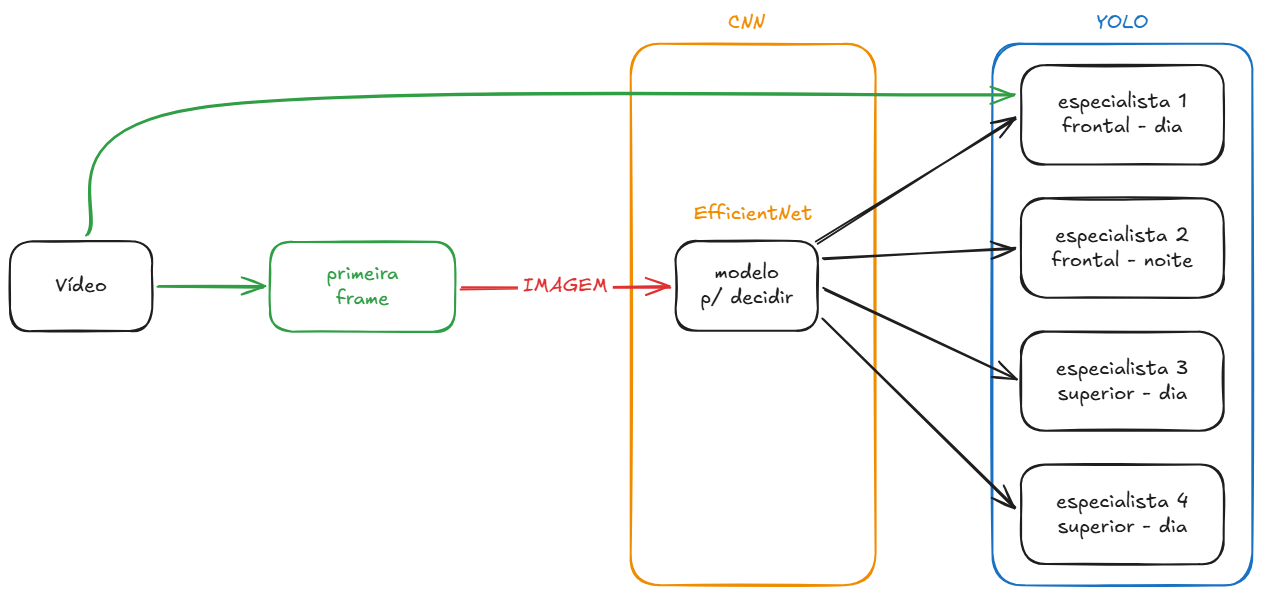
\includegraphics[width=\textwidth]{figs/moe.png}
\caption{Arquitetura MoE proposta: o primeiro quadro do vídeo é classificado pela rede de roteamento (EfficientNet-B0), que seleciona um dos quatro especialistas YOLOv8m; o especialista selecionado processa todos os quadros do vídeo.}
\label{fig:arquitetura-moe}

Fonte: Elaborada pelo autor.
\end{figure}

O \textit{pipeline} recebe um vídeo e executa os seguintes passos:
\begin{enumerate}
    \item O primeiro quadro do vídeo é lido e convertido para o espaço de cores RGB;
    \item O quadro passa pelo mesmo pré-processamento da validação da rede de roteamento (redimensionamento, recorte central em 224$\times$224 pixels e normalização do ImageNet) e é classificado pela EfficientNet-B0. As saídas da rede passam por uma função \textit{softmax}, e o cenário de maior probabilidade é escolhido; essa probabilidade é registrada como a confiança do roteamento;
    \item Os pesos do especialista correspondente ao cenário escolhido são carregados;
    \item O especialista processa todos os quadros do vídeo, com limiar de confiança de 0,7 e limiar de IoU de 0,7 para a supressão de não máximos (\textit{non-maximum suppression}, NMS), que elimina caixas sobrepostas atribuídas a um mesmo objeto;
    \item O vídeo anotado com as caixas detectadas e um relatório com o cenário identificado, a confiança do roteamento, o especialista usado e o tempo de processamento são salvos.
\end{enumerate}

O roteamento é feito uma única vez por vídeo, no primeiro quadro. Essa escolha parte do fato de que as câmeras são fixas: a perspectiva de um vídeo nunca muda, e a iluminação de uma sessão curta normalmente também não. Com isso, a rede de roteamento é executada uma vez, e o custo por quadro é o de um único YOLOv8m, igual ao do baseline. Em contrapartida, um erro de roteamento no primeiro quadro compromete o vídeo inteiro, e uma sessão que atravessasse o amanhecer ou o anoitecer continuaria a ser processada pelo especialista escolhido no início. O roteamento quadro a quadro, ou em intervalos regulares, eliminaria essa limitação ao custo de executar a rede de roteamento mais vezes.

\section{Avaliação em Vídeos de Teste}
\label{sec:avaliacao-videos}

\subsection{Vídeos de Teste e Verificação de Vazamento}
\label{subsec:videos-teste}

Além da validação cruzada, as duas abordagens foram avaliadas em quatro vídeos de teste, um por cenário, com 80 quadros cada (10 segundos a 8 FPS). Esses vídeos foram gravados na mesma baia. Os vídeos Frontal Dia e Frontal Noite vêm da câmera Cam03, e os vídeos Superior Dia e Superior Noite, da câmera Cam04.

Como os arquivos de teste não traziam metadados de data e hora nem seguiam o padrão de nome das sessões, foi preciso confirmar que nenhum deles era um recorte de uma sessão de treino. A verificação teve duas etapas. Na primeira, a data indicada no nome de cada vídeo foi comparada com as datas das sessões de treino. Essa comparação serve apenas como indício, pois várias sessões de câmeras diferentes podem ter a mesma data. Na segunda etapa, que é a decisiva, foram amostrados 12 quadros de cada vídeo de teste e comparados com as imagens de treino das sessões candidatas (as de mesma data ou, se nenhuma data coincidisse, todas as sessões). A comparação usou primeiro um \textit{hash} médio (\textit{average hash}) de 8$\times$8 bits, que descarta rapidamente pares muito diferentes: só seguiram para a etapa seguinte os pares com distância de Hamming de no máximo 12 bits. Os pares restantes foram comparados pelo erro quadrático médio (\textit{mean squared error}, MSE) entre os pixels das duas imagens, redimensionadas para 160$\times$160 pixels:
\begin{equation}
    \mathrm{MSE}(I, J) = \frac{1}{N} \sum_{k=1}^{N} \left( I_k - J_k \right)^2,
    \label{eq:mse}
\end{equation}
em que $I_k$ e $J_k$ são os valores do $k$-ésimo pixel e canal das duas imagens, e $N$ é o número total de valores.

O limiar de decisão foi calibrado na própria base. O MSE de uma imagem com ela mesma é zero, e o MSE entre dois quadros diferentes de uma mesma sessão de treino ficou entre cerca de 750 e 1.200, já que os animais se movem entre um quadro e outro. Um quadro de teste foi considerado duplicata de um quadro de treino apenas se o menor MSE encontrado fosse de no máximo 60, valor compatível com a diferença causada por uma nova compressão do mesmo quadro, e não com a de duas cenas parecidas. Como o pré-filtro por \textit{hash} pode descartar pares que, comparados pelo MSE, seriam próximos, a verificação foi repetida de forma exaustiva: todos os 80 quadros de cada vídeo de teste foram comparados, pelo MSE, com todas as imagens da base de detecção vindas da mesma câmera. Além disso, a câmera, a data e a hora gravadas na própria imagem pelo sistema de gravação foram lidas no primeiro quadro de cada vídeo de teste e comparadas com o intervalo de tempo coberto por cada sessão da base, obtido da mesma marcação no primeiro e no último quadro da sessão. Os resultados dessa verificação são apresentados no Capítulo~5.

\subsection{Protocolo de Inferência e Métrica de Contagem}
\label{subsec:metrica-contagem}

Os quatro vídeos foram processados pelo \textit{pipeline} MoE (Seção~\ref{sec:arquitetura-moe}) e pelo baseline monolítico, com o mesmo limiar de confiança (0,7), o mesmo limiar de IoU da supressão de não máximos (0,7) e a mesma resolução de entrada (640$\times$640 pixels).

Os vídeos de teste não têm rótulos, de modo que não é possível calcular precisão, revocação ou mAP sobre eles. A avaliação usou, em vez disso, a contagem de caixas. Como os oito animais estão sempre na baia, um detector sem erros produz exatamente oito caixas em cada quadro, ou $8 \times 80 = 640$ caixas por vídeo. Para cada abordagem e cada vídeo, foram registrados o total de caixas, o número de caixas por quadro e os quadros com menos ou mais de oito caixas. Menos de oito caixas indica animais não detectados; mais de oito indica detecções duplicadas ou falsos positivos.

A contagem total é uma medida grosseira, pois um animal perdido e uma caixa duplicada no mesmo quadro se compensam. Por isso, a análise também considerou a distribuição da contagem quadro a quadro e, nos quadros com mais de oito caixas, o IoU entre pares de caixas, para verificar se as caixas excedentes eram duplicatas sobre um mesmo animal que a supressão de não máximos deixou passar. Também foram registradas a confiança da rede de roteamento em cada vídeo e a faixa de confiança das caixas produzidas pelos especialistas. Os quadros com erros foram inspecionados visualmente, lado a lado, para as duas abordagens.

\section{Ambiente Computacional}
\label{sec:ambiente-computacional}

Os experimentos foram executados em um computador com sistema operacional Linux, processador de 16 núcleos e uma GPU NVIDIA GeForce RTX 5070 com 12 GB de memória. A base de imagens ficou armazenada em discos rígidos mecânicos. O código foi escrito em Python, em um ambiente Conda, com as bibliotecas PyTorch e \textit{torchvision} (rede de roteamento), Ultralytics (treinamento e inferência dos detectores YOLOv8), Captum (análise de oclusão), OpenCV (leitura de vídeos e extração de quadros), scikit-learn (divisão da base da rede de roteamento e métricas de classificação) e pandas, Matplotlib e seaborn (análise dos resultados e geração de gráficos).

%%%%%%%%%%%%%%%%%%%%%%%%%%%%%%%%%%%%%%%%%%%%%%%%%%%%%%%%%%%
%
%--------------CAPÍTULO 5 - RESULTADOS E DISCUSSÃO----------
%
%
\chapter{Resultados e Discussão}
\label{cap:resultados}

Este capítulo apresenta os resultados na ordem em que as etapas foram executadas (Capítulo~\ref{cap:materiais-metodos}). A Seção~\ref{sec:res-poc} mostra o resultado da prova de conceito com o detector pré-treinado. A Seção~\ref{sec:res-roteamento} apresenta o treinamento da rede de roteamento e a análise de seus mapas de oclusão. As Seções~\ref{sec:res-especialistas} e~\ref{sec:res-baseline} trazem as métricas de validação cruzada dos especialistas e do baseline monolítico, e a Seção~\ref{sec:res-comparacao-metricas} compara as duas abordagens com base nessas métricas. A Seção~\ref{sec:res-videos} apresenta a avaliação nos vídeos de teste independentes, e a Seção~\ref{sec:res-discussao} discute o conjunto dos resultados e suas limitações.

\section{Prova de Conceito com Detector Pré-Treinado}
\label{sec:res-poc}

A Figura~\ref{fig:poc-sheep} mostra o resultado típico do YOLOv8m pré-treinado no COCO aplicado a um quadro da câmera frontal durante o dia, com as detecções filtradas pela classe \textit{sheep}. Dos oito animais da baia principal, o modelo detectou apenas dois, com confianças de 0,27 e 0,48. Os testes com imagens noturnas e com a perspectiva superior também tiveram desempenho insatisfatório, sem que o modelo detectasse o rebanho completo.

\begin{figure}[htb]
\centering
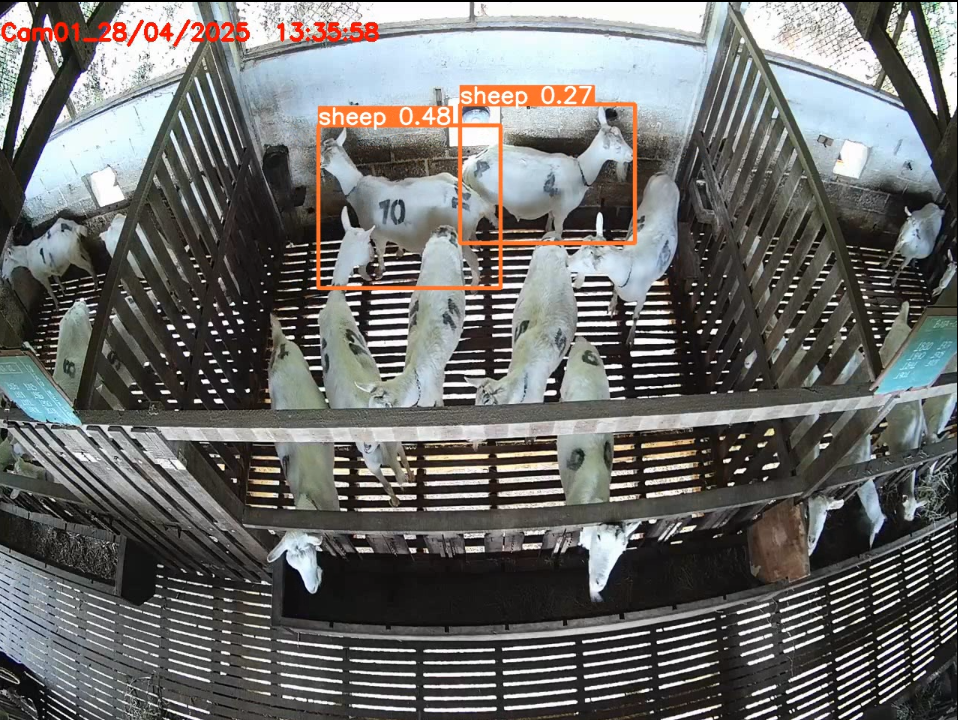
\includegraphics[width=0.75\textwidth]{figs/sheep-test.png}
\caption{Prova de conceito: YOLOv8m pré-treinado no COCO, sem ajuste, com detecções filtradas pela classe \textit{sheep}. Apenas dois dos oito animais da baia principal foram detectados.}
\label{fig:poc-sheep}

Fonte: Elaborada pelo autor.
\end{figure}

Esse desempenho era esperado. O COCO não tem caprinos, e cabras \textit{Saanen} vistas de cima ou em diagonal, através das grades de uma baia, têm aparência diferente da dos ovinos que o modelo aprendeu a reconhecer. À noite, a diferença aumenta, porque as imagens em infravermelho são monocromáticas, ao passo que o COCO é formado por fotografias coloridas. O teste confirmou que seria necessário construir uma base própria e treinar detectores para o domínio. Como teve caráter apenas exploratório, esse teste não é usado como base de comparação no restante do capítulo; esse papel cabe ao baseline monolítico (Seção~\ref{sec:res-baseline}).

\section{Rede de Roteamento}
\label{sec:res-roteamento}

\subsection{Treinamento e Desempenho de Validação}
\label{subsec:res-treino-roteamento}

O treinamento da EfficientNet-B0 foi interrompido pela parada antecipada na nona época. A Figura~\ref{fig:curva-roteamento} mostra a perda de treino e de validação ao longo das épocas. A perda de validação ficou próxima de zero já a partir da segunda época e não voltou a cair o suficiente para reiniciar a contagem da paciência, o que levou à parada sete épocas depois. A perda de treino oscilou mais, com picos na quarta e na sexta épocas, efeito esperado do aumento de dados aplicado só ao treino, e também se aproximou de zero nas últimas épocas.

\begin{figure}[htb]
\centering
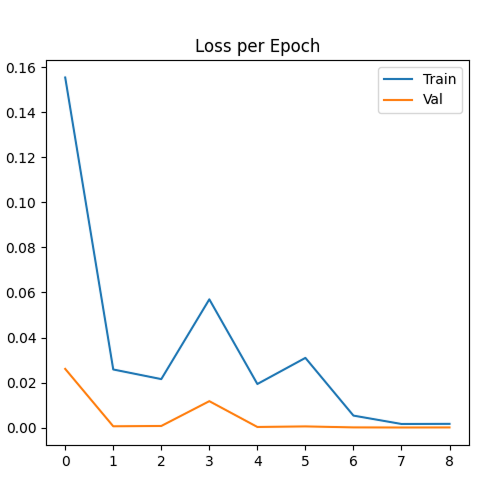
\includegraphics[width=0.5\textwidth]{figs/learning_curves.png}
\caption{Perda de treino (\textit{Train}) e de validação (\textit{Val}) da rede de roteamento por época. A numeração das épocas no eixo horizontal começa em zero.}
\label{fig:curva-roteamento}

Fonte: Elaborada pelo autor.
\end{figure}

No conjunto de validação, com 272 imagens, a rede classificou corretamente todas as imagens dos quatro cenários: precisão, revocação e F1-\textit{score} foram iguais a 1,00 em todas as classes. A convergência rápida e o acerto total indicam que distinguir os quatro cenários é uma tarefa fácil para a rede. Isso faz sentido, já que a diferença entre perspectiva frontal e superior muda a geometria inteira da cena, e a diferença entre dia e noite muda a cor da imagem inteira.

Esse resultado precisa ser lido com cautela por dois motivos já apontados na Seção~\ref{subsec:base-roteamento}. O primeiro é que a divisão entre treino e validação dessa base foi aleatória por quadro, de modo que quadros próximos de um mesmo vídeo podem estar nos dois conjuntos. O segundo é que a base é desbalanceada, e a classe Frontal Noite tem apenas 16 imagens de validação. O acerto total, portanto, não prova que a rede generalize para vídeos novos. Essa verificação é feita na Seção~\ref{subsec:res-roteamento-videos}, com os vídeos de teste independentes.

\subsection{Mapas de Sensibilidade por Oclusão}
\label{subsec:res-oclusao}

A Figura~\ref{fig:oclusao} mostra os mapas de sensibilidade por oclusão de uma imagem de cada cenário, sobrepostos às imagens. As cores quentes (amarelo e vermelho) indicam as regiões cuja oclusão mais altera a saída da rede para a classe prevista, e as cores frias (azul), as regiões que pouco influenciam a decisão. A rede previu corretamente o cenário das quatro imagens.

\begin{figure}[htb]
\centering
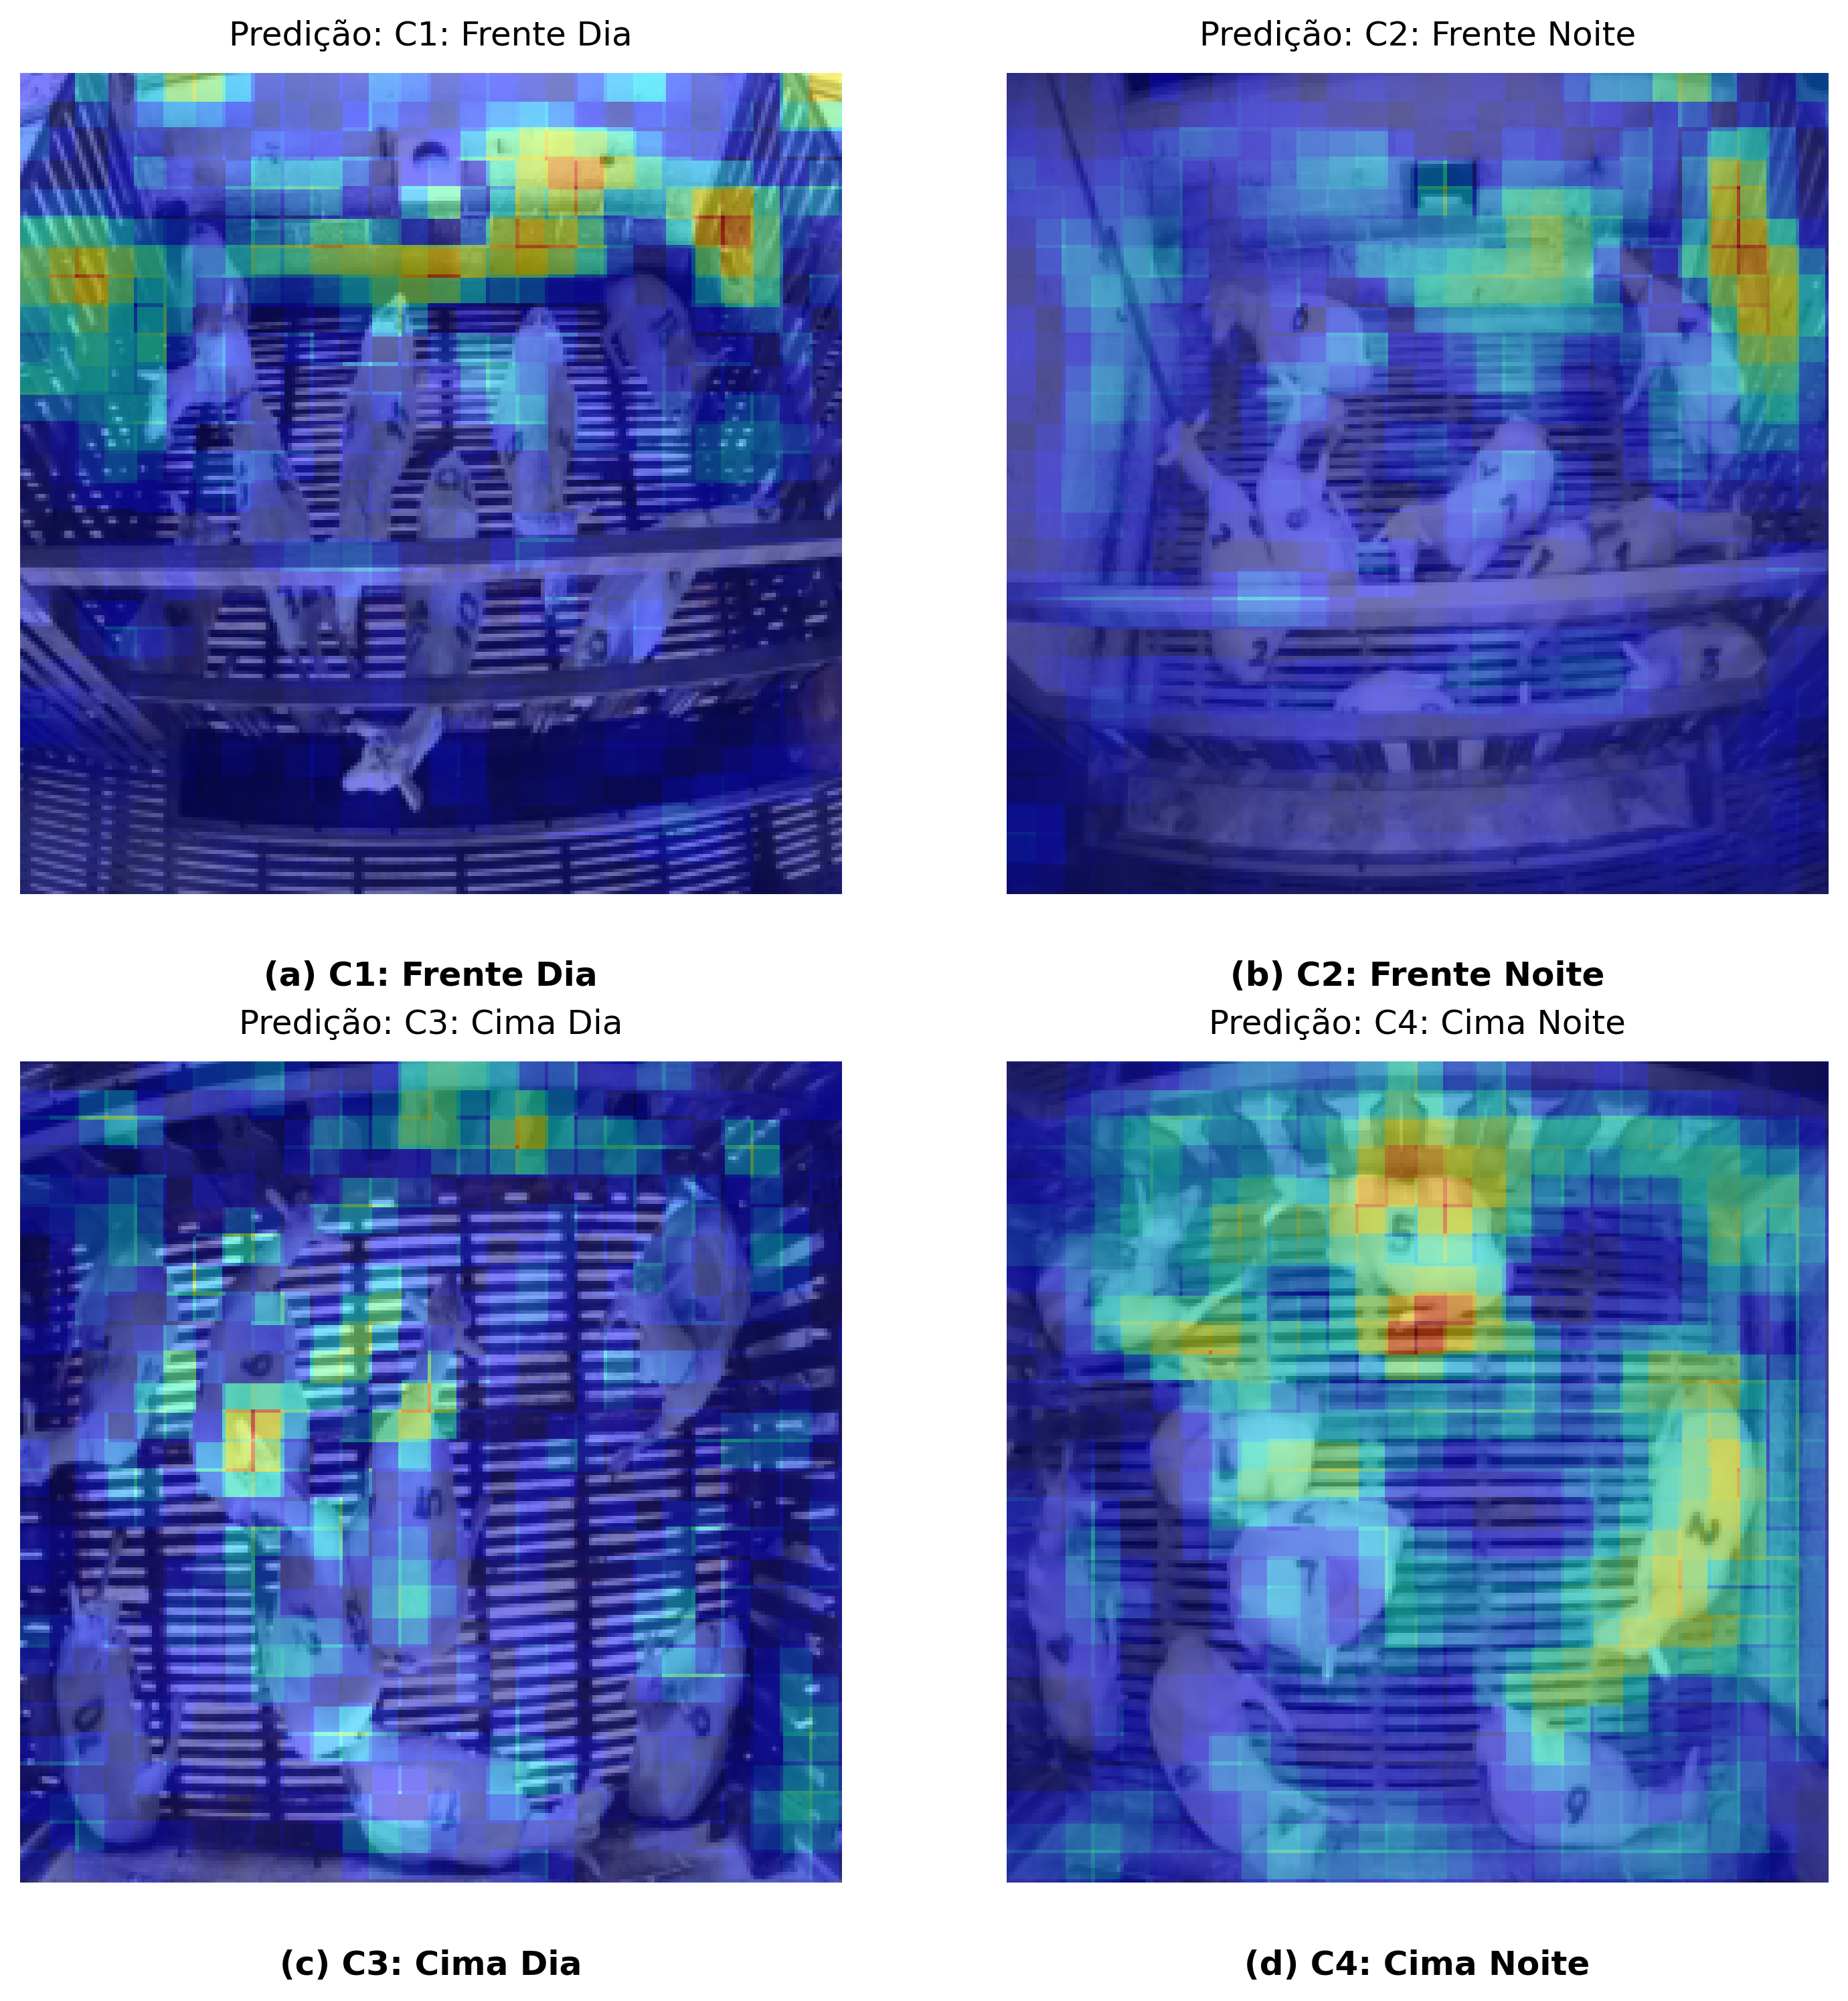
\includegraphics[width=0.85\textwidth]{figs/occlusion_2x2_blended.png}
\caption{Mapas de sensibilidade por oclusão da rede de roteamento, sobrepostos às imagens de entrada: (a) Frontal Dia; (b) Frontal Noite; (c) Superior Dia; (d) Superior Noite. Cores quentes indicam maior influência na decisão.}
\label{fig:oclusao}

Fonte: Elaborada pelo autor.
\end{figure}

Nos dois cenários frontais, a rede se apoiou sobretudo na estrutura da baia. Em Frontal Dia (Figura~\ref{fig:oclusao}a), as regiões mais relevantes ficam na faixa superior da imagem, sobre a parede do fundo e a parte alta das grades laterais, e quase não há relevância sobre os corpos dos animais ou sobre o cocho na parte inferior. Em Frontal Noite (Figura~\ref{fig:oclusao}b), o padrão é parecido: a região mais relevante é a grade do lado direito e a parte superior da parede, enquanto os animais aparecem em azul.

Nos cenários superiores, o padrão é menos uniforme. Em Superior Dia (Figura~\ref{fig:oclusao}c), o mapa é difuso: há pontos de relevância moderada espalhados sobre o piso ripado e a borda superior da imagem, sem uma região dominante. Em Superior Noite (Figura~\ref{fig:oclusao}d), a região de maior relevância fica no centro da imagem e coincide em parte com o corpo de dois animais e com o piso entre eles. Nesse caso, a rede não se baseou apenas no cercado e nas paredes.

Os mapas indicam que, na maioria dos casos, a rede usa elementos fixos da cena para reconhecer o cenário, como as paredes, as grades e o piso, que mudam de aparência entre as perspectivas e entre o dia e a noite. O caso Superior Noite mostra, porém, que os animais também podem pesar na decisão. Isso não chega a ser um problema para o roteamento, já que a aparência dos animais em infravermelho e vistos de cima também é característica do cenário, mas significa que a afirmação de que a rede ``olha apenas para o ambiente'' não vale para todos os casos. A análise cobre uma imagem por cenário e tem caráter qualitativo; uma conclusão mais geral exigiria aplicar a oclusão a um conjunto maior de imagens.

\section{Detectores Especialistas}
\label{sec:res-especialistas}

A Tabela~\ref{tab:res-especialistas} apresenta, para cada especialista, as métricas do melhor \textit{fold}, escolhido pelo maior mAP50 (Seção~\ref{sec:especialistas}). A coluna ``Época'' indica a época em que esse mAP50 foi atingido.

\begin{table}[htb]
\centering
\caption{Métricas de validação do melhor \textit{fold} de cada especialista (época de maior mAP50).}
\label{tab:res-especialistas}
\begin{tabular}{lccccccc}
\hline
\textbf{Especialista} & \textbf{Fold} & \textbf{Época} & \textbf{P} & \textbf{R} & \textbf{F1} & \textbf{mAP50} & \textbf{mAP50-95} \\
\hline
Frontal Dia & 2 & 108 & 0,9966 & 0,9975 & 0,9971 & 0,9950 & 0,9015 \\
Frontal Noite & 3 & 81 & 0,9972 & 0,9968 & 0,9970 & 0,9950 & 0,8821 \\
Superior Dia & 4 & 50 & 0,9999 & 0,9995 & 0,9997 & 0,9950 & 0,8645 \\
Superior Noite & 5 & 13 & 0,9978 & 0,9972 & 0,9975 & 0,9950 & 0,8338 \\
\hline
\end{tabular}

\vspace{0.2cm}
Fonte: Elaborada pelo autor.
\end{table}

Os quatro especialistas atingiram mAP50 de 0,9950, e a precisão, a revocação e o F1-\textit{score} ficaram acima de 0,99 em todos os casos. Com um limiar de IoU de 0,5, portanto, praticamente todos os animais dos blocos de validação foram encontrados, com pouquíssimos falsos positivos. O mAP50 de 0,9950 é, na prática, o valor máximo que essa métrica atinge na implementação usada, e todos os \textit{folds} de todos os especialistas chegaram a ele ou ficaram a uma diferença na terceira ou quarta casa decimal. Por isso, o mAP50 não diferencia os especialistas entre si, e a escolha do melhor \textit{fold} por esse critério é praticamente um desempate.

A métrica mais exigente, o mAP50-95, separa os cenários. Os especialistas frontais tiveram os maiores valores (0,9015 em Frontal Dia e 0,8821 em Frontal Noite), seguidos por Superior Dia (0,8645) e Superior Noite (0,8338). A perspectiva superior, portanto, foi a mais difícil para o ajuste fino das caixas. Uma explicação plausível é que, vistos de cima, os animais ficam muito próximos uns dos outros, sobretudo junto ao cocho, e as bordas de um animal encostam nas do vizinho, o que torna mais difícil acertar a caixa com IoU alto. O mesmo padrão aparece nos dois períodos do dia: em cada perspectiva, o cenário noturno teve mAP50-95 menor que o diurno.

As épocas da Tabela~\ref{tab:res-especialistas} variam bastante, de 13 em Superior Noite a 108 em Frontal Dia. Elas não devem ser lidas como uma medida da velocidade de convergência de cada especialista. Como o mAP50 satura muito cedo, a época em que ele atinge seu valor máximo depende de pequenas oscilações na quarta casa decimal. Além disso, o mAP50-95 continua a subir depois dessa época, como mostra a Seção~\ref{sec:res-baseline} para o baseline. O valor de mAP50-95 da tabela é, portanto, o daquela época específica, e tende a ser menor que o dos pesos efetivamente salvos pela biblioteca, que são escolhidos pela métrica de aptidão. A Tabela~\ref{tab:res-especialistas-aptidao} mostra as métricas na época de maior aptidão, que no Ultralytics é o próprio mAP50-95. São esses os pesos que a biblioteca salva e que o \textit{pipeline} MoE usa. Como no baseline (Seção~\ref{sec:res-baseline}), todos os 20 treinamentos pararam exatamente 30 épocas depois da época de maior aptidão. A última coluna traz a média do mAP50-95 dos cinco \textit{folds} de cada especialista, no mesmo critério.

\begin{table}[htb]
\centering
\caption{Especialistas na época de maior aptidão (pesos salvos): \textit{fold} usado no \textit{pipeline}, época de parada, duração do treinamento e média do mAP50-95 dos cinco \textit{folds}.}
\label{tab:res-especialistas-aptidao}
\footnotesize
\begin{tabular}{lccccccc}
\hline
\textbf{Especialista} & \textbf{Fold} & \shortstack{\textbf{Época}\\\textbf{(aptidão)}} & \textbf{mAP50} & \textbf{mAP50-95} & \textbf{Parada} & \textbf{Duração} & \shortstack{\textbf{mAP50-95}\\\textbf{(média)}} \\
\hline
Frontal Dia & 2 & 102 & 0,9949 & 0,9068 & 132 & 38 min & 0,9017 \\
Frontal Noite & 3 & 52 & 0,9949 & 0,8875 & 82 & 21 min & 0,8835 \\
Superior Dia & 4 & 92 & 0,9950 & 0,8738 & 122 & 45 min & 0,8421 \\
Superior Noite & 5 & 58 & 0,9950 & 0,8706 & 88 & 26 min & 0,8968 \\
\hline
\end{tabular}

\vspace{0.2cm}
\normalsize
Fonte: Elaborada pelo autor.
\end{table}

Nesse critério, o mAP50-95 de todos os especialistas sobe em relação à Tabela~\ref{tab:res-especialistas}, e a ordenação entre os cenários muda. A maior diferença está em Superior Noite: o \textit{fold} escolhido passa de 0,8338 (época 13) para 0,8706, e a média dos cinco \textit{folds} desse especialista (0,8968) fica abaixo apenas da de Frontal Dia. O padrão em que o cenário noturno tem mAP50-95 menor que o diurno da mesma perspectiva, portanto, era em boa parte efeito da época de maior mAP50. O que se mantém nos dois critérios é que Superior Dia tem o menor mAP50-95 médio. Os 20 treinamentos dos especialistas somaram cerca de 13 horas e 50 minutos.

\section{Baseline Monolítico}
\label{sec:res-baseline}

A Tabela~\ref{tab:res-baseline} apresenta as métricas do baseline em cada \textit{fold}, segundo o mesmo critério dos especialistas (época de maior mAP50).

\begin{table}[htb]
\centering
\caption{Métricas de validação do baseline monolítico por \textit{fold} (época de maior mAP50).}
\label{tab:res-baseline}
\begin{tabular}{lcccccc}
\hline
\textbf{Fold} & \textbf{Época} & \textbf{P} & \textbf{R} & \textbf{F1} & \textbf{mAP50} & \textbf{mAP50-95} \\
\hline
1 & 96 & 0,9914 & 0,9938 & 0,9926 & 0,9944 & 0,8700 \\
2 & 60 & 0,9945 & 0,9942 & 0,9943 & 0,9948 & 0,8707 \\
3 & 54 & 0,9977 & 0,9986 & 0,9982 & 0,9950 & 0,8965 \\
4 & 33 & 0,9967 & 0,9971 & 0,9969 & 0,9950 & 0,8839 \\
5 & 25 & 0,9939 & 0,9948 & 0,9943 & 0,9949 & 0,8653 \\
\hline
\textbf{Média} & -- & \textbf{0,9948} & \textbf{0,9957} & \textbf{0,9953} & \textbf{0,9948} & \textbf{0,8773} \\
\hline
\end{tabular}

\vspace{0.2cm}
Fonte: Elaborada pelo autor.
\end{table}

O baseline também satura o mAP50, entre 0,9944 e 0,9950 nos cinco \textit{folds}, e tem precisão e revocação médias acima de 0,99. O mAP50-95 varia mais entre os \textit{folds}, de 0,8653 a 0,8965, com média de 0,8773. Como os \textit{folds} diferem apenas no trecho de cada sessão reservado para validação, essa variação mostra que alguns trechos das gravações são mais difíceis que outros, por exemplo por concentrarem momentos em que os animais estão agrupados.

A Figura~\ref{fig:curvas-baseline} mostra a evolução do mAP50 e do mAP50-95 ao longo do treinamento dos cinco \textit{folds}. O mAP50 (Figura~\ref{fig:curvas-baseline}a) chega a cerca de 0,995 nas primeiras épocas e praticamente não muda depois disso. O mAP50-95 (Figura~\ref{fig:curvas-baseline}b) sobe rapidamente nas primeiras dezenas de épocas e continua crescendo lentamente por muito mais tempo. Os círculos vazados marcam a época de maior mAP50, usada nas Tabelas~\ref{tab:res-especialistas} e~\ref{tab:res-baseline}, e os círculos cheios marcam a época de maior aptidão, cujos pesos a biblioteca salva. Em todos os \textit{folds}, o círculo cheio fica à direita e acima do vazado.

\begin{figure}[htb]
\centering
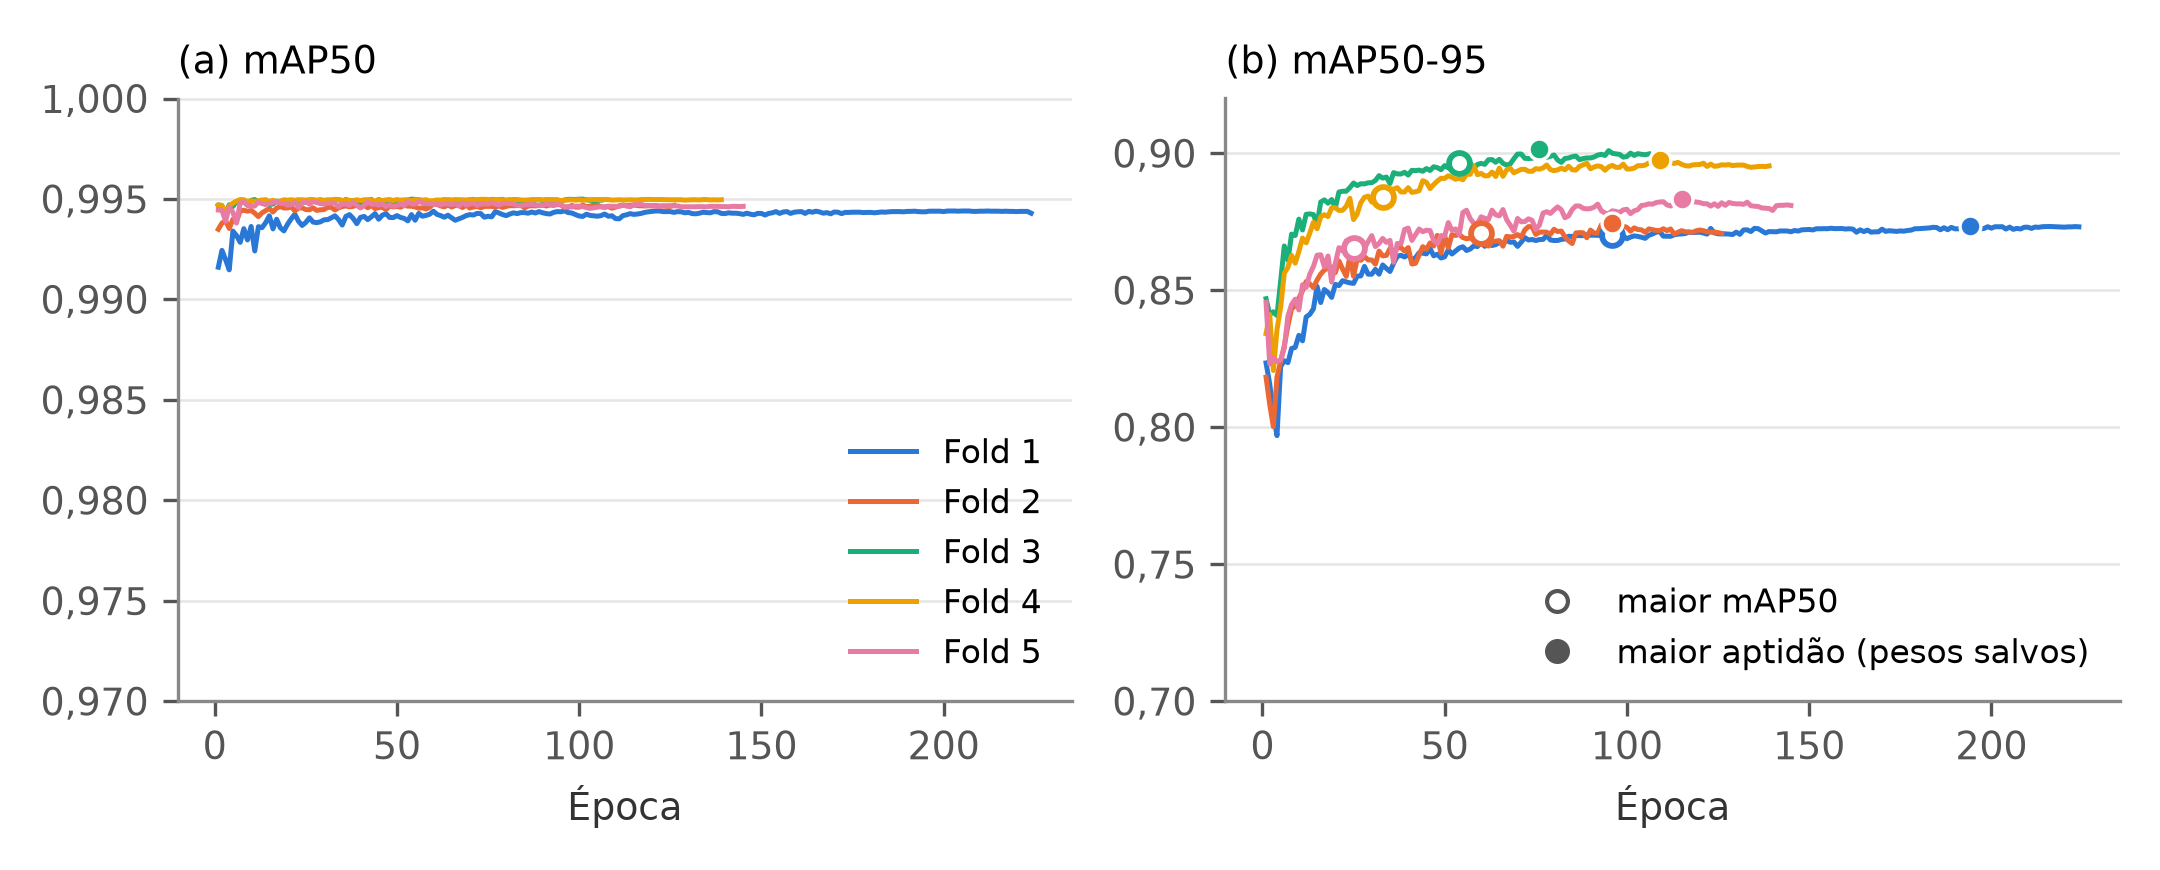
\includegraphics[width=\textwidth]{figs/baseline_curvas.png}
\caption{Evolução do mAP50 (a) e do mAP50-95 (b) de validação do baseline monolítico nos cinco \textit{folds}. Em (b), os círculos vazados indicam a época de maior mAP50 e os círculos cheios, a época de maior aptidão (pesos salvos).}
\label{fig:curvas-baseline}

Fonte: Elaborada pelo autor.
\end{figure}

A Tabela~\ref{tab:res-baseline-aptidao} mostra as métricas na época de maior aptidão, junto com a época em que cada treinamento parou e sua duração. A parada ocorreu sempre 30 épocas depois da época de maior aptidão, o que confirma que a paciência foi contada sobre essa métrica. Nesse critério, o mAP50-95 médio do baseline sobe de 0,8773 para 0,8860, e o do \textit{fold} 3 chega a 0,9015. Os cinco treinamentos somaram cerca de 15 horas.

\begin{table}[htb]
\centering
\caption{Baseline monolítico na época de maior aptidão (pesos salvos), época de parada e duração do treinamento de cada \textit{fold}.}
\label{tab:res-baseline-aptidao}
\footnotesize
\begin{tabular}{lccccc}
\hline
\textbf{Fold} & \textbf{Época (aptidão)} & \textbf{mAP50} & \textbf{mAP50-95} & \textbf{Parada} & \textbf{Duração} \\
\hline
1 & 194 & 0,9944 & 0,8733 & 224 & 4 h 39 min \\
2 & 96 & 0,9946 & 0,8745 & 126 & 2 h 29 min \\
3 & 76 & 0,9950 & 0,9015 & 106 & 2 h 05 min \\
4 & 109 & 0,9949 & 0,8974 & 139 & 2 h 45 min \\
5 & 115 & 0,9947 & 0,8832 & 145 & 3 h 05 min \\
\hline
\textbf{Média} & -- & \textbf{0,9947} & \textbf{0,8860} & -- & \textbf{15 h 03 min} (total) \\
\hline
\end{tabular}

\vspace{0.2cm}
\normalsize
Fonte: Elaborada pelo autor.
\end{table}

\section{Comparação entre Especialistas e Baseline nas Métricas Agregadas}
\label{sec:res-comparacao-metricas}

Nas métricas de validação cruzada, as duas abordagens têm desempenho muito parecido. Ambas saturam o mAP50 e têm precisão, revocação e F1-\textit{score} acima de 0,99. No mAP50-95, os especialistas variam de 0,8338 a 0,9015, e o baseline tem média de 0,8773 e melhor \textit{fold} com 0,8965.

Essa comparação, porém, não é direta, por três motivos. Primeiro, os números dos especialistas são os do melhor \textit{fold} de cada um, enquanto o valor de referência do baseline é a média dos cinco \textit{folds}; comparar o melhor caso de uma abordagem com a média da outra favorece a primeira. Comparando melhor \textit{fold} com melhor \textit{fold}, o baseline (0,8965) supera três dos quatro especialistas no mAP50-95 e fica abaixo apenas de Frontal Dia (0,9015). Segundo, cada especialista é avaliado apenas sobre o seu cenário, enquanto o baseline é avaliado sobre a união dos quatro; o mAP50-95 do baseline é uma média que mistura cenários mais fáceis e mais difíceis. Terceiro, como discutido nas seções anteriores, as tabelas usam a época de maior mAP50, que não corresponde aos pesos salvos.

A forma mais justa de comparar as duas abordagens é avaliar o baseline separadamente sobre a validação de cada cenário, no mesmo \textit{fold} e com os pesos salvos, e comparar cenário a cenário com o especialista correspondente. Essa comparação é possível porque o conjunto de validação do baseline em cada \textit{fold} é exatamente a união dos conjuntos de validação dos quatro especialistas no mesmo \textit{fold}: o particionamento foi gerado pelo mesmo procedimento, sessão a sessão, e as 8.604 imagens caem no mesmo bloco nos dois casos. Os pesos salvos (\texttt{best.pt}) de cada \textit{fold} do baseline foram então avaliados pela rotina de validação do Ultralytics, com os parâmetros padrão, sobre o subconjunto de validação de cada cenário. Como verificação, a mesma avaliação sobre a validação completa reproduziu, até a quarta casa decimal, o mAP50-95 registrado pelo treinamento na época de maior aptidão (Tabela~\ref{tab:res-baseline-aptidao}). Do lado dos especialistas, foram usadas as métricas da época de maior aptidão de cada \textit{fold}, que correspondem aos pesos salvos. A Tabela~\ref{tab:res-comparacao-cenario} resume o resultado.

\begin{table}[htb]
\centering
\caption{mAP50-95 de validação por cenário: especialista e baseline monolítico avaliados sobre o mesmo subconjunto de validação, no mesmo \textit{fold}, com os pesos salvos (média $\pm$ desvio padrão dos cinco \textit{folds}).}
\label{tab:res-comparacao-cenario}
\footnotesize
\begin{tabular}{lcccc}
\hline
\textbf{Cenário} & \textbf{Especialista} & \textbf{Baseline} & \shortstack{\textbf{Diferença}\\\textbf{(esp. $-$ base)}} & \shortstack{\textbf{\textit{Folds} com}\\\textbf{especialista melhor}} \\
\hline
Frontal Dia & 0,9017 $\pm$ 0,0042 & 0,9061 $\pm$ 0,0078 & $-$0,0044 & 1 de 5 \\
Frontal Noite & 0,8835 $\pm$ 0,0061 & 0,8859 $\pm$ 0,0078 & $-$0,0025 & 1 de 5 \\
Superior Dia & 0,8421 $\pm$ 0,0268 & 0,8477 $\pm$ 0,0291 & $-$0,0055 & 0 de 5 \\
Superior Noite & 0,8968 $\pm$ 0,0390 & 0,9101 $\pm$ 0,0284 & $-$0,0133 & 1 de 5 \\
\hline
\end{tabular}

\vspace{0.2cm}
\normalsize
Fonte: Elaborada pelo autor.
\end{table}

No mAP50, as duas abordagens continuam empatadas em todos os cenários (médias entre 0,9941 e 0,9949). No mAP50-95, o baseline teve média ligeiramente maior que o especialista nos quatro cenários e foi melhor em 17 dos 20 pares de \textit{fold} e cenário. As diferenças são pequenas, entre 0,0025 e 0,0133, menores que a variação entre \textit{folds} de um mesmo modelo nos cenários superiores, mas têm sempre o mesmo sinal. A conclusão, portanto, é que a arquitetura MoE não demonstra superioridade sobre o baseline nas métricas agregadas de detecção; na comparação cenário a cenário, é o baseline que fica levemente à frente. No regime de dados deste trabalho, um único YOLOv8m consegue aprender uma representação conjunta das quatro combinações de perspectiva e iluminação tão boa quanto, ou ligeiramente melhor que, a de cada especialista, possivelmente porque é treinado com quatro vezes mais imagens.

\section{Avaliação em Vídeos de Teste}
\label{sec:res-videos}

\subsection{Verificação de Vazamento}
\label{subsec:res-vazamento}

A Tabela~\ref{tab:res-vazamento} mostra o resultado da verificação de vazamento descrita na Seção~\ref{subsec:videos-teste}. Na primeira rodada, feita com o pré-filtro por \textit{hash}, nenhum dos quatro vídeos foi identificado como recorte de uma sessão de treino: nos três vídeos em que algum par passou pelo pré-filtro, o menor MSE ficou entre 1.326,8 e 2.546,8, e no vídeo Superior Dia nenhum par passou. Essa rodada, porém, tinha duas fragilidades. O pré-filtro comparava apenas 12 quadros do vídeo com uma amostra das imagens de cada sessão e podia descartar pares próximos, e a escolha das sessões candidatas dependia da data escrita no nome do arquivo de teste, que estava errada no vídeo Superior Noite (o nome indica 29 de abril, mas a marcação gravada nos quadros indica 26 de abril). A tabela apresenta, por isso, o resultado da verificação exaustiva, que compara todos os quadros com todas as imagens da mesma câmera, e a comparação da marcação de hora dos vídeos com o intervalo coberto por cada sessão.

\begin{table}[htb]
\centering
\caption{Verificação de vazamento entre os vídeos de teste e as sessões da base de detecção (busca exaustiva por MSE contra todas as imagens da mesma câmera).}
\label{tab:res-vazamento}
\footnotesize
\begin{tabular}{lcccc}
\hline
\shortstack{\textbf{Vídeo}\\\textbf{de teste}} & \shortstack{\textbf{Câmera,}\\\textbf{data e hora}} & \shortstack{\textbf{Sessão que cobre}\\\textbf{o horário}} & \shortstack{\textbf{Menor}\\\textbf{MSE}} & \textbf{Resultado} \\
\hline
Frontal Dia & Cam03, 04/05, 14h10 & nenhuma & 1.232,3 & sem vazamento \\
Frontal Noite & Cam03, 26/04, 18h40 & Cam03, 26/04, 18h17--19h16 & 11,9 & mesma sessão \\
Superior Dia & Cam04, 29/04, 12h50 & nenhuma & 2.148,6 & sem vazamento \\
Superior Noite & Cam04, 26/04, 20h45 & nenhuma & 941,4 & sem vazamento \\
\hline
\end{tabular}

\vspace{0.2cm}
\normalsize
Fonte: Elaborada pelo autor.
\end{table}

Em três vídeos, o resultado se confirma. Os vídeos Frontal Dia e Superior Dia foram gravados em dias sem nenhuma sessão da mesma câmera na base. O vídeo Superior Noite foi gravado às 20h45 de 26 de abril, e as três sessões da Cam04 nesse dia cobrem os intervalos de 0h07 a 1h06, de 4h06 a 5h06 e de 18h06 a 19h05; o vídeo começa, portanto, 1 hora e 40 minutos depois do fim da sessão mais próxima, e o menor MSE (941,4) está na faixa de duas cenas diferentes.

O vídeo Frontal Noite, por outro lado, é um trecho de uma sessão da base. A sessão \texttt{Cam03\_2025\_04\_26\_18\_17\_10} não é um trecho contínuo de poucos segundos: seus 140 quadros cobrem uma hora de gravação, das 18h17 às 19h16, e o vídeo de teste, gravado às 18h40, está dentro desse intervalo. O quadro 54 da sessão, registrado às 18h40min17s, 4 segundos depois do último quadro do vídeo, tem MSE de 11,9 em relação a ele, abaixo do limiar de duplicata. A primeira rodada não detectou esse caso porque o pré-filtro não levou esse par à comparação por MSE. Nos \textit{folds} 1, 4 e 5, esse quadro está no treino; no \textit{fold} 3, cujos pesos foram usados tanto pelo especialista Frontal Noite quanto pelo baseline nos testes em vídeo, ele está na validação, e a imagem de treino mais próxima do vídeo é o quadro 40 da mesma sessão, cerca de seis minutos antes, com MSE de 85,2. Não há, portanto, quadro idêntico ao do vídeo no treino dos modelos testados, mas o vídeo vem da mesma gravação, com a mesma câmera, a mesma iluminação e os animais em posições parecidas. O vídeo Frontal Noite não é, assim, um teste independente, e o resultado da contagem nesse cenário deve ser lido como o de um trecho de uma sessão vista no treino. Como as duas abordagens usaram o mesmo \textit{fold} e, portanto, as mesmas imagens dessa sessão no treino, a comparação entre elas nesse vídeo continua sendo feita em condições iguais.

\subsection{Roteamento}
\label{subsec:res-roteamento-videos}

A rede de roteamento escolheu o cenário correto nos quatro vídeos. A confiança da escolha, isto é, a probabilidade atribuída pela \textit{softmax} ao cenário escolhido, foi de 99,32\% em Frontal Dia, 99,38\% em Superior Dia e 99,99\% em Superior Noite. Em Frontal Noite, foi de apenas 62,67\%.

Mesmo correta, uma confiança de 62,67\% indica que, para o primeiro quadro desse vídeo, a rede distribuiu uma parte considerável da probabilidade entre outros cenários. Isso mostra que o acerto total na validação (Seção~\ref{subsec:res-treino-roteamento}) superestima a margem de segurança da rede em vídeos novos, e que o roteamento feito com base em um único quadro tem, nesse cenário, pouca folga. Um fator que pode contribuir é que Frontal Noite é a classe com menos imagens na base da rede de roteamento (80, contra 560 de Frontal Dia).

Para investigar esse caso, a rede de roteamento foi aplicada novamente ao primeiro quadro e a todos os 80 quadros de cada vídeo de teste. No primeiro quadro do vídeo Frontal Noite, a probabilidade restante foi para Superior Noite (31,4\%), Frontal Dia (5,2\%) e Superior Dia (0,6\%). A confiança baixa não é uma particularidade desse quadro: a rede escolheu Frontal Noite em todos os 80 quadros do vídeo, mas sempre com confiança entre 58,5\% e 62,7\%, e sempre com cerca de 30\% para Superior Noite. Nos outros três vídeos, a confiança ficou acima de 98,6\% em todos os quadros. O quadro também não tem nada de incomum: a exposição é normal, e os animais estão no centro da baia, longe da câmera.

A explicação mais provável está na base da rede de roteamento (Seção~\ref{subsec:base-roteamento}). A classe Frontal Noite foi treinada com um único vídeo de 10 segundos da câmera Cam01, enquanto o vídeo de teste vem da câmera Cam03, que nenhuma imagem da base de roteamento representa. As duas câmeras frontais estão em posições diferentes e têm enquadramentos diferentes da baia. À noite, sem a informação de cor, a distinção entre as perspectivas depende só da geometria da cena, e um enquadramento que a rede não viu no treino pode ficar, para ela, a meio caminho entre as duas classes noturnas. De dia, a mesma câmera Cam03 foi classificada com mais de 98\% de confiança, possivelmente porque a classe Frontal Dia tem sete vídeos e porque a cor ajuda a separar os cenários. Como a confiança é baixa de forma sistemática em todos os quadros, classificar vários quadros e decidir pela média das probabilidades não aumentaria a margem nesse vídeo, embora proteja contra um primeiro quadro atípico. A forma de tornar o roteamento mais seguro é incluir na base de roteamento imagens de todas as câmeras usadas, em especial da Cam03 e da Cam04.

\subsection{Contagem de Animais}
\label{subsec:res-contagem}

A Tabela~\ref{tab:res-contagem} apresenta o total de caixas detectadas por cada abordagem em cada vídeo. Como os oito animais estão na baia em todos os quadros, o valor esperado é de 640 caixas por vídeo.

\begin{table}[htb]
\centering
\caption{Total de caixas detectadas nos vídeos de teste (80 quadros cada; valor esperado de $8 \times 80 = 640$).}
\label{tab:res-contagem}
\begin{tabular}{lccc}
\hline
\textbf{Cenário} & \textbf{Baseline} & \textbf{MoE} & \textbf{Esperado} \\
\hline
Frontal Dia & 623 & 640 & 640 \\
Frontal Noite & 643 & 640 & 640 \\
Superior Dia & 532 & 640 & 640 \\
Superior Noite & 663 & 640 & 640 \\
\hline
\end{tabular}

\vspace{0.2cm}
Fonte: Elaborada pelo autor.
\end{table}

A arquitetura MoE produziu exatamente 640 caixas nos quatro vídeos, com oito caixas em cada um dos 320 quadros. O baseline errou a contagem nos quatro vídeos, ora para menos, ora para mais. A análise quadro a quadro mostra dois padrões de erro diferentes.

O primeiro é a subdetecção. No vídeo Superior Dia, o baseline não chegou a oito caixas em nenhum dos 80 quadros, oscilando entre cinco e sete, e o total ficou 108 caixas abaixo do esperado. Nesse vídeo, os animais aparecem agrupados e encostados uns nos outros, e o baseline tende a deixar de fora animais parcialmente encobertos pelos vizinhos. No vídeo Frontal Dia, o total ficou 17 caixas abaixo do esperado.

O segundo é a sobredetecção. No vídeo Superior Noite, 26 dos 80 quadros tiveram mais de oito caixas, chegando a dez, e no vídeo Frontal Noite isso ocorreu em 4 dos 80 quadros. Nesses quadros, as caixas excedentes não são falsos positivos sobre o fundo: são caixas duplicadas sobre um animal que já tinha sido detectado. O IoU entre a caixa duplicada e a original chegou a 0,64, abaixo do limiar de 0,7 da supressão de não máximos, de modo que as duas caixas foram mantidas pelo pós-processamento. Nos totais da Tabela~\ref{tab:res-contagem}, a sobredetecção pode encobrir parte da subdetecção; o total de Frontal Noite (643), por exemplo, está próximo do esperado, mas inclui quadros com caixas a mais.

A Figura~\ref{fig:comparacao-videos} mostra exemplos desses erros, com o baseline à esquerda e o especialista correspondente à direita, no mesmo quadro de cada vídeo. Em Frontal Dia (a, b) e Superior Dia (e, f), o baseline detecta seis e cinco animais, respectivamente, e o especialista detecta os oito. Em Frontal Noite (c, d) e Superior Noite (g, h), o baseline atribui duas caixas a um mesmo animal, ambas com confiança de pelo menos 0,73, enquanto o especialista delimita cada animal com uma única caixa.

\begin{figure}[p]
\centering
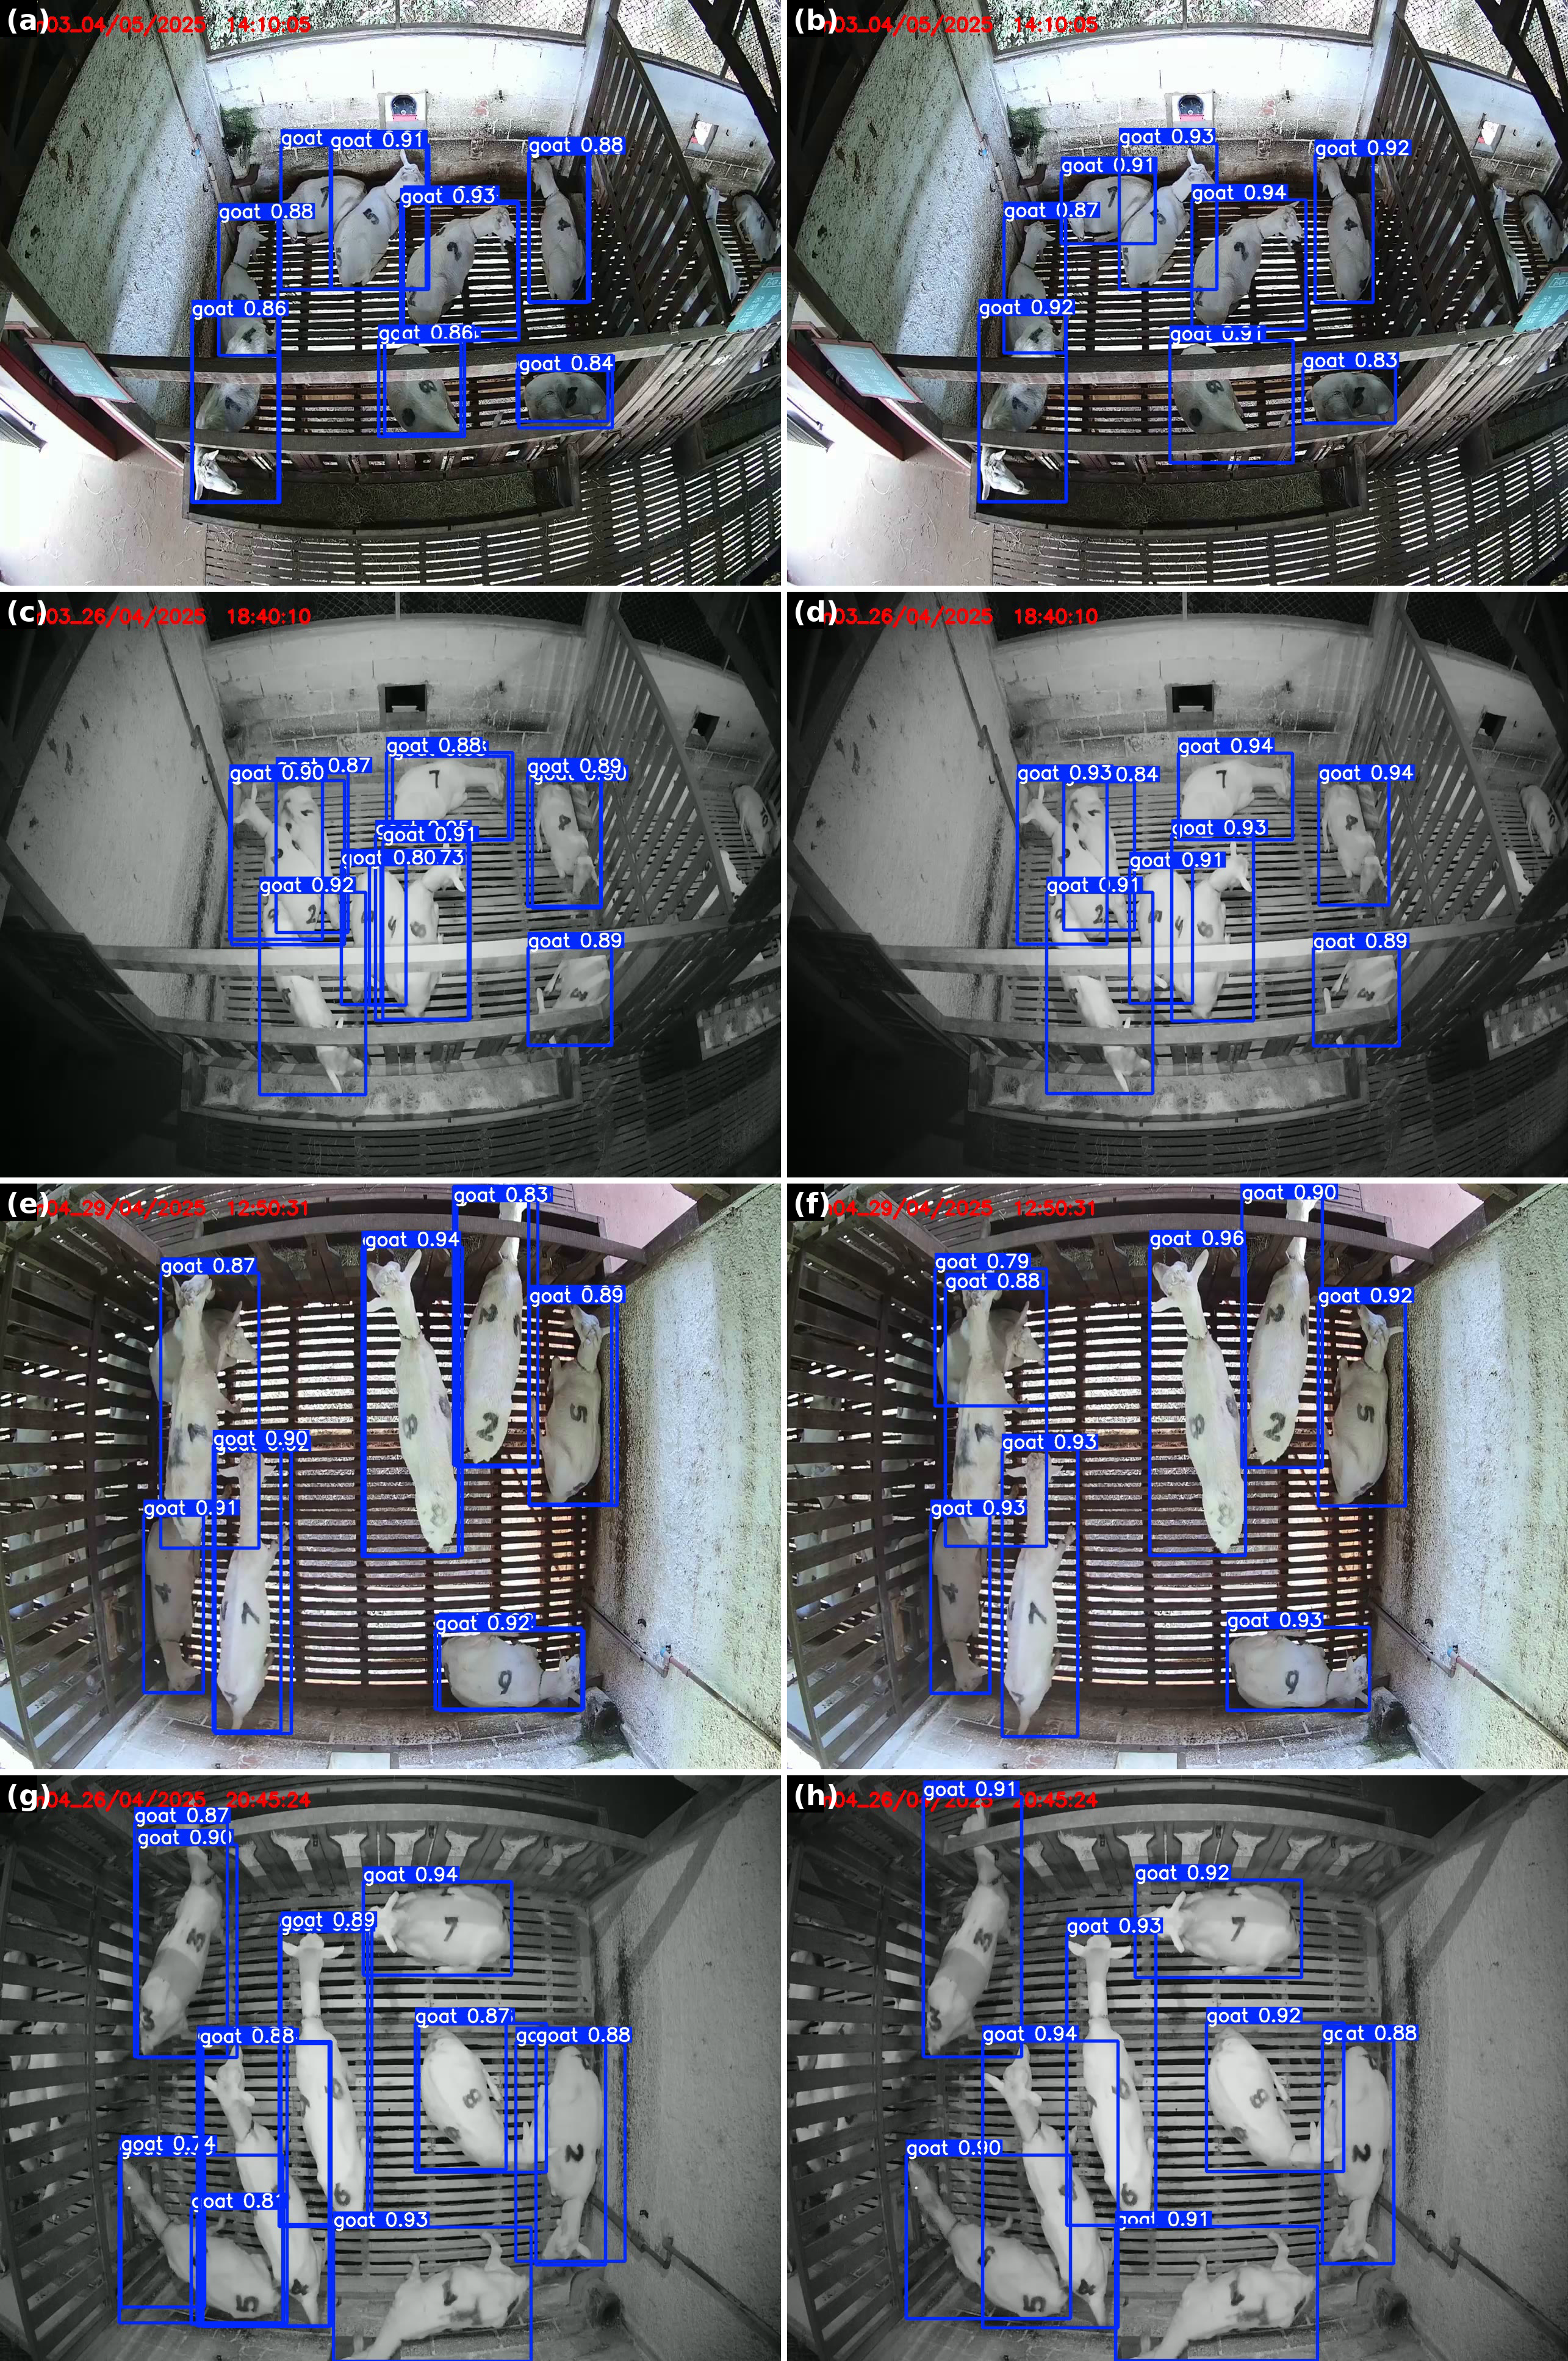
\includegraphics[width=0.82\textwidth]{figs/comparacao_overall_moe.png}
\caption{Baseline monolítico (esquerda) e especialista MoE correspondente (direita), no mesmo quadro do mesmo vídeo de teste: (a)-(b) Frontal Dia, quadro 10 (6 e 8 caixas); (c)-(d) Frontal Noite, quadro 55 (9 e 8 caixas); (e)-(f) Superior Dia, quadro 62 (5 e 8 caixas); (g)-(h) Superior Noite, quadro 6 (10 e 8 caixas).}
\label{fig:comparacao-videos}

Fonte: Elaborada pelo autor.
\end{figure}

As 2.560 caixas produzidas pelos especialistas nos quatro vídeos tiveram confiança entre 0,74 e 0,96, com média de 0,91. Como o limiar de confiança usado foi 0,7, nenhuma caixa ficou muito perto do limite de corte, o que indica que a contagem correta não dependeu de um ajuste fino desse limiar.

\section{Discussão}
\label{sec:res-discussao}

\subsection{Por que as Métricas Agregadas não Mostram a Diferença}
\label{subsec:disc-metricas}

Os resultados das Seções~\ref{sec:res-comparacao-metricas} e~\ref{sec:res-videos} parecem contraditórios. Nas métricas de validação cruzada, as duas abordagens empatam; na contagem em vídeo, o baseline erra nos quatro cenários e o MoE acerta todos os quadros. Há duas razões principais para essa diferença.

A primeira é que as duas avaliações medem coisas diferentes. O mAP resume a qualidade do detector em todos os limiares de confiança, ordenando as caixas da mais confiante para a menos confiante. Uma caixa duplicada sobre um animal já detectado conta como um falso positivo, mas, se tiver confiança menor que a das caixas corretas, entra no fim dessa ordenação e reduz pouco a área sob a curva de precisão e revocação. Na contagem, em um limiar fixo de 0,7, a mesma caixa duplicada soma um animal a mais no quadro. Do mesmo modo, um animal detectado com confiança 0,6 contribui para o mAP, mas desaparece da contagem com o limiar de 0,7.

A segunda é que os vídeos de teste são mais distantes do treino que os blocos de validação. Como discutido na Seção~\ref{subsec:limitacoes-protocolo}, a validação usa trechos de sessões cujos outros trechos foram vistos no treino. Os vídeos de teste vêm de momentos diferentes, com outras posições e agrupamentos dos animais, com a exceção do vídeo Frontal Noite, que é um trecho de uma sessão da base (Seção~\ref{subsec:res-vazamento}). É razoável supor que, diante de dados realmente novos, as diferenças entre as abordagens apareçam mais do que na validação cruzada, e foi o que se observou.

\subsection{Interpretação do Desempenho dos Especialistas}
\label{subsec:disc-especialistas}

Os especialistas mantiveram a contagem correta nos quatro cenários, inclusive naqueles em que o baseline mais errou. Uma interpretação compatível com esses resultados é que cada especialista, treinado com imagens de uma única combinação de perspectiva e iluminação, ajusta o tamanho e a forma das caixas e o nível de confiança a uma distribuição visual mais homogênea. O baseline precisa conciliar, nos mesmos parâmetros, animais grandes e vistos de lado nas câmeras frontais com animais menores e vistos de cima nas câmeras superiores, em imagens coloridas e em infravermelho. Os erros do baseline foram diferentes em cada cenário (subdetecção nos cenários diurnos, sobredetecção nos noturnos), o que é coerente com um modelo cujo ajuste é um compromisso entre cenários. Essa interpretação, no entanto, não foi testada diretamente, e outros fatores, como diferenças entre os \textit{folds} escolhidos, podem contribuir para o resultado.

\subsection{Vantagens e Custos da Arquitetura Modular}
\label{subsec:disc-modularidade}

Além da estabilidade da contagem, a arquitetura MoE tem propriedades estruturais que as métricas não medem. Um novo cenário, como uma nova câmera ou uma nova baia, pode ser incorporado treinando um novo especialista e acrescentando uma classe à rede de roteamento, sem retreinar os especialistas existentes. Uma dificuldade própria de um cenário, como o mAP50-95 mais baixo da perspectiva superior, fica restrita ao especialista daquele cenário e pode ser tratada nele, por exemplo com mais dados, sem risco de piorar os demais. E a rede de roteamento informa, para cada vídeo, qual especialista foi usado e com que confiança, um sinal que pode ser registrado e auditado e que não existe em um detector único.

Esses benefícios têm custos. O sistema tem cinco modelos em vez de um, e o treinamento dos especialistas e da rede de roteamento exige mais etapas que o de um detector único. O roteamento é um ponto único de falha: um erro no primeiro quadro leva o vídeo inteiro a um especialista inadequado, e o caso de Frontal Noite mostrou que a margem da rede de roteamento pode ser pequena em vídeos novos. No custo de inferência, as duas abordagens se equivalem, pois executam um único YOLOv8m por quadro, e a rede de roteamento é executada apenas uma vez por vídeo. Nos testes, tanto o \textit{pipeline} MoE quanto o baseline processaram cada vídeo de 80 quadros em menos de 3 segundos na GPU usada nos experimentos; esses tempos podem incluir o aquecimento inicial do modelo e não foram medidos de forma controlada, e não foram feitas medições em equipamentos de menor capacidade.

\subsection{Limitações}
\label{subsec:disc-limitacoes}

Os resultados deste capítulo devem ser lidos com as seguintes limitações. A validação cruzada não separa sessões inteiras entre treino e validação, e a validação da rede de roteamento foi feita com divisão aleatória por quadro. As métricas das Tabelas~\ref{tab:res-especialistas} e~\ref{tab:res-baseline} correspondem à época de maior mAP50, e não aos pesos salvos, embora a comparação cenário a cenário (Tabela~\ref{tab:res-comparacao-cenario}) use os pesos salvos. A avaliação em vídeo usou um único vídeo por cenário, com 80 quadros cada, sem rótulos, e o vídeo Frontal Noite pertence a uma sessão da base de detecção. A base da rede de roteamento não contém imagens das câmeras Cam03 e Cam04, de onde vêm os vídeos de teste. Além disso, a métrica de contagem não distingue um animal perdido de um compensado por uma caixa duplicada no mesmo quadro. Por fim, toda a base vem de uma única baia, com o mesmo rebanho de oito animais, e o comportamento dos modelos em outras instalações não foi avaliado. Essas limitações não invalidam o padrão observado, que foi consistente nos quatro cenários, mas restringem o alcance das conclusões e orientam os trabalhos futuros discutidos no Capítulo~6.

%%%%%%%%%%%%%%%%%%%%%%%%%%%%%%%%%%%%%%%%%%%%%%%%%%%%%%%%%%%
%
%--------------CAPÍTULO 6 - CONCLUSÃO-----------------------
%
%
\chapter{Conclusão}
\label{cap:conclusao}

Este trabalho investigou a detecção automática de caprinos da raça \textit{Saanen} em uma baia de confinamento monitorada por câmeras fixas, sob duas perspectivas (frontal e superior) e duas condições de iluminação (diurna e noturna, em infravermelho). Para lidar com essa variação, foi proposta uma arquitetura de Mistura de Especialistas em que uma rede de roteamento baseada na EfficientNet-B0 identifica o cenário de captura no primeiro quadro do vídeo e seleciona um de quatro detectores YOLOv8m, cada um treinado com as imagens de um único cenário. A arquitetura foi comparada com um baseline monolítico, um único YOLOv8m treinado com a união das imagens dos quatro cenários, sob o mesmo protocolo de validação.

\section{Síntese dos Resultados}
\label{sec:sintese-resultados}

A pergunta de pesquisa apresentada no Capítulo~\ref{cap:introducao} foi se seria possível detectar caprinos de forma robusta em um confinamento sujeito a variações de perspectiva e iluminação, avaliando os modelos sob um protocolo que reduzisse o vazamento temporal. Os resultados indicam que sim, com as ressalvas discutidas na Seção~\ref{sec:limitacoes}. A seguir, retoma-se cada objetivo específico.

O primeiro objetivo era construir e caracterizar uma base de imagens rotuladas. A base final reúne 8.604 imagens e 66.705 caixas delimitadoras da classe \texttt{goat}, extraídas de 36 sessões de gravação em sete dias, e está organizada pelos quatro cenários de captura, com tamanhos parecidos entre eles (de 2.001 a 2.549 imagens). Cada imagem preserva a câmera, a sessão e a posição do quadro na gravação, informação que tornou possível o protocolo de validação adotado.

O segundo objetivo era definir um protocolo de validação que reduzisse o vazamento temporal. O protocolo de validação cruzada por blocos temporais divide cada sessão em cinco trechos contíguos e exclui do treino as 15 imagens vizinhas de cada borda do bloco de validação. A auditoria confirmou que nenhuma imagem aparece ao mesmo tempo em treino e validação, e a zona de exclusão removeu 4.234 amostras somando os cinco \textit{folds}. O protocolo substituiu o particionamento aleatório das primeiras rodadas de experimentos, cujas métricas estavam infladas pela presença de quadros quase idênticos em treino e validação.

O terceiro objetivo era treinar e avaliar detectores para os cenários considerados. Os quatro especialistas atingiram mAP50 de 0,9950 e precisão, revocação e F1-\textit{score} acima de 0,99. No mAP50-95, os especialistas frontais tiveram os maiores valores (0,9015 em Frontal Dia e 0,8821 em Frontal Noite) e os superiores, os menores (0,8645 em Superior Dia e 0,8338 em Superior Noite), o que aponta a perspectiva superior, em que os animais aparecem agrupados e encostados, como a mais difícil para o ajuste fino das caixas.

O quarto objetivo era investigar a identificação automática do cenário e a interpretabilidade dessa decisão. A rede de roteamento acertou todas as 272 imagens de validação e escolheu o cenário correto nos quatro vídeos de teste. Os mapas de oclusão mostraram que, nos cenários frontais, a decisão se apoia sobretudo na estrutura da baia, como paredes e grades, enquanto em Superior Noite os animais também pesam na decisão. No vídeo Frontal Noite, a confiança do roteamento foi de 62,67\%, bem abaixo dos demais vídeos, o que mostra que a margem da rede em vídeos novos é menor do que o acerto total na validação sugere.

O quinto objetivo era integrar os componentes em um \textit{pipeline} de inferência. O \textit{pipeline} recebe um vídeo, classifica o primeiro quadro, carrega o especialista correspondente e processa todos os quadros, registrando o cenário identificado, a confiança do roteamento e as detecções. Como a rede de roteamento é executada uma vez por vídeo, o custo por quadro é o de um único YOLOv8m, o mesmo do baseline.

O sexto objetivo era comparar a abordagem proposta com um detector não especializado. Nas métricas de validação cruzada, as duas abordagens tiveram desempenho muito próximo: o baseline também satura o mAP50 e tem mAP50-95 médio de 0,8773, e seu melhor \textit{fold} supera três dos quatro especialistas nessa métrica. A arquitetura MoE, portanto, não se mostrou superior nas métricas agregadas. A diferença apareceu na contagem de animais nos vídeos de teste independentes: a arquitetura MoE detectou exatamente os oito animais em todos os 320 quadros, enquanto o baseline errou a contagem nos quatro cenários, com subdetecção nos vídeos diurnos (até 108 caixas a menos em Superior Dia) e caixas duplicadas sobre um mesmo animal nos noturnos (26 dos 80 quadros com mais de oito caixas em Superior Noite).

Em conjunto, os resultados indicam que a vantagem da especialização por cenário, neste problema, não está no mAP, mas na estabilidade do detector em vídeos novos, além das propriedades estruturais da arquitetura modular: a possibilidade de incluir novos cenários sem retreinar os especialistas existentes, o isolamento das dificuldades de cada cenário em seu próprio especialista e o registro explícito de qual especialista foi usado em cada vídeo.

\section{Contribuições}
\label{sec:contribuicoes-finais}

As principais contribuições deste trabalho são:
\begin{itemize}
    \item uma base de 8.604 imagens de caprinos \textit{Saanen} em confinamento, anotadas com 66.705 caixas e organizadas por perspectiva e iluminação, incluindo imagens noturnas em infravermelho, um tipo de dado pouco presente nas bases públicas da área;
    \item um protocolo de validação cruzada por blocos temporais com zona de exclusão, aplicável a outros trabalhos que usam quadros extraídos de vídeo, acompanhado de uma auditoria do particionamento;
    \item uma arquitetura de Mistura de Especialistas com roteamento por cenário de captura, com a análise da decisão de roteamento por oclusão;
    \item uma comparação entre a arquitetura especializada e um detector único treinado sob o mesmo protocolo, que mostra que métricas agregadas de validação podem não revelar diferenças que aparecem na contagem de animais em vídeo.
\end{itemize}

\section{Limitações}
\label{sec:limitacoes}

As conclusões acima estão sujeitas a limitações discutidas ao longo dos Capítulos~4 e~5. O protocolo de validação reduz o vazamento entre quadros vizinhos, mas não separa sessões inteiras entre treino e validação, e a base da rede de roteamento foi dividida aleatoriamente por quadro. As métricas tabeladas correspondem à época de maior mAP50, e não aos pesos efetivamente salvos, e a comparação entre especialistas e baseline nas métricas agregadas não foi feita cenário a cenário. A avaliação em vídeo usou um vídeo por cenário, com 80 quadros, sem rótulos, e a verificação de vazamento do vídeo Superior Noite precisa ser refeita contra as sessões da data correta. Toda a base provém de uma única baia e de um único rebanho de oito animais, e o desempenho em outras instalações não foi avaliado. Por fim, não foram feitas medições de desempenho em equipamentos de menor capacidade computacional, de modo que este trabalho não permite afirmar a viabilidade da solução em dispositivos embarcados.

\section{Trabalhos Futuros}
\label{sec:trabalhos-futuros}

As limitações apontadas sugerem uma primeira linha de trabalhos, voltada a tornar a avaliação mais rigorosa:
\begin{itemize}
    \item adotar um particionamento por sessão ou por dia de aquisição (\textit{Group K-Fold}) para os detectores e para a rede de roteamento, à medida que a base ganhe mais sessões por cenário;
    \item comparar especialistas e baseline cenário a cenário, avaliando o baseline sobre a validação de cada cenário e usando, nos dois casos, os pesos efetivamente salvos;
    \item ampliar o conjunto de teste para vários vídeos por cenário, com rótulos, de modo a medir precisão, revocação e erro de contagem quadro a quadro sobre dados independentes;
    \item avaliar os modelos em outras baias e com outros rebanhos.
\end{itemize}

Uma segunda linha diz respeito à própria arquitetura. O roteamento pode ser tornado mais seguro classificando vários quadros do início do vídeo, ou repetindo a classificação em intervalos regulares, o que também permitiria lidar com sessões que atravessem o amanhecer ou o anoitecer. A causa da baixa confiança do roteamento no vídeo Frontal Noite deve ser investigada, e a base da rede de roteamento pode ser ampliada e balanceada, em especial nessa classe. A sobredetecção do baseline sugere ainda testar o efeito do limiar de IoU da supressão de não máximos nas duas abordagens. Também vale medir o tempo de inferência e o consumo de memória de forma controlada, inclusive em equipamentos de menor capacidade, para avaliar a viabilidade de execução junto às câmeras.

Por fim, este trabalho corresponde ao módulo de detecção do projeto ``Inteligência artificial aplicada à detecção e classificação comportamental de cabras em confinamento (raça \textit{Saanen})''. As etapas seguintes do projeto partem das detecções produzidas aqui: o rastreamento de cada animal ao longo do vídeo (\textit{multi-object tracking}) e a classificação de comportamentos como alimentação, ócio e deslocamento, que permitirão usar o sistema no acompanhamento do bem-estar do rebanho.


%%%%%%%%%%%%%%%%%%%%%%%%%%%%%%%%%%%%%%%
\singlespacing
\bibliographystyle{abntex2-alf}
\bibliography{referencias}

%%%%%%%%%%%%%%%%%%%%%%%%%%%%%%%%%%%%%%%%%%%%%%%%

\end{document}
